%Fred, Simon, Sou-Cheng, Yuhan, NSF Grant Sep 2021
% GitHub: https://github.com/fjhickernell/NSF_CompMath2018Nov
% Overleaf: https://www.overleaf.com/9576964687whkhbmrrvhsd
\documentclass[11pt]{NSFamsart}
\usepackage{latexsym,amsfonts,amsmath,amssymb,amsthm,epsfig,extdash,multirow}
\usepackage{stackrel,tabularx,mathtools,longtable,xspace}
\usepackage[shortlabels]{enumitem}
\usepackage[dvipsnames]{xcolor}
\usepackage[numbers,sort&compress]{natbib}
\usepackage{hyperref}
\usepackage{accents, booktabs}
\usepackage{algorithm, algorithmicx}
\usepackage{anyfontsize}
\usepackage{cleveref}
\usepackage{wrapfig}
\usepackage[font=small,labelfont=bf]{caption}

\voffset 0.2in
\textheight 9in
\textwidth6.5in
\setlength{\oddsidemargin}{0in}
\setlength{\evensidemargin}{0in}
%\thispagestyle{empty} \pagestyle{empty} %to eliminate page numbers for upload
\thispagestyle{plain} \pagestyle{plain} %to add back page numbers

\headsep-0.6in


\usepackage{minted}
\newminted{python}{frame=lines,framerule=1.5pt,breaklines=true}
\newmintinline[pyinline]{python}{}


\usepackage{algpseudocode}
\algnewcommand\algorithmicparam{\textbf{Parameters:}}
\algnewcommand\PARAM{\item[\algorithmicparam]}
\algnewcommand\algorithmicinput{\textbf{Input:}}
\algnewcommand\INPUT{\item[\algorithmicinput]}
%\algnewcommand\STATE{\item}
\algnewcommand\RETURN{\State \textbf{Return }}

%\usepackage{showlabels}
\newcommand{\Upara}[1]{\noindent\underline{#1}:\xspace}

\newcommand{\myshade}{60}
\colorlet{mylinkcolor}{violet}
\colorlet{mycitecolor}{violet}
%\colorlet{mycitecolor}{OliveGreen}
\colorlet{myurlcolor}{YellowOrange}

\hypersetup{
	linkcolor  = mylinkcolor!\myshade!black,
	citecolor  = mycitecolor!\myshade!black,
	urlcolor   = myurlcolor!\myshade!black,
	colorlinks = true,
}


% This package prints the labels in the margin
%\usepackage[notref,notcite]{showkeys}


%%list of acronyms with links
\newcommand{\FH}{\hyperlink{FHlink}{FH}\xspace}
\newcommand{\SM}{\hyperlink{SMlink}{SM}\xspace}
\newcommand{\SCTC}{\hyperlink{SCTClink}{SCTC}\xspace}
\newcommand{\AO}{\hyperlink{AOlink}{AO}\xspace}
\newcommand{\MM}{\hyperlink{MMlink}{MM}\xspace}
\newcommand{\TS}{\hyperlink{TSlink}{TS}\xspace}
\newcommand{\GEF}{\hyperlink{GEFlink}{GEF}\xspace}
\newcommand{\YD}{\hyperlink{YDlink}{YD}\xspace}
\newcommand{\JR}{\hyperlink{JRlink}{JR}\xspace}
\newcommand{\LlAJR}{\hyperlink{LlAJRlink}{LlAJR}\xspace}
\newcommand{\LJ}{\hyperlink{LJlink}{LJ}\xspace}
\newcommand{\XT}{\hyperlink{XTlink}{XT}\xspace}
\newcommand{\KZ}{\hyperlink{KZlink}{KZ}\xspace}
\newcommand{\DL}{\hyperlink{DLlink}{DL}\xspace}
\newcommand{\XZ}{\hyperlink{XZlink}{KZ}\xspace}
\newcommand{\JL}{\hyperlink{JLlink}{JL}\xspace}
\newcommand{\YZ}{\hyperlink{YZlink}{YZ}\xspace}
\newcommand{\AS}{\hyperlink{ASlink}{AS}\xspace}
\newcommand{\CLT}{\hyperlink{CLTlink}{CLT}\xspace}
\newcommand{\PN}{\hyperlink{PNlink}{PN}\xspace}
\newcommand{\PR}{\hyperlink{PRlink}{PR}\xspace}
\newcommand{\DN}{\hyperlink{DNlink}{DN}\xspace}


\newcommand{\QMCSoft}{QMCSoft\xspace}
\newcommand{\GAIL}{GAIL\xspace}
\newcommand{\QMC}{QMC\xspace}
\newcommand{\IIDMC}{IID MC\xspace}
\newcommand{\SAMSIQMC}{SAMSI-QMC\xspace}
\newcommand{\SciPy}{SciPy\xspace}
\newcommand{\GSL}{GSL\xspace}
\newcommand{\NAG}{NAG\xspace}
\newcommand{\MATLAB}{MATLAB\xspace}
\newcommand{\Chebfun}{Chebfun\xspace}
\newcommand{\Rlang}{R\xspace}
\newcommand{\Julia}{Julia\xspace}


%\textheight9.1in

\newtheorem{theorem}{theorem}


\providecommand{\FJHickernell}{Hickernell}
\newcommand{\hf}{\widehat{f}}
\newcommand{\hg}{\widehat{g}}
\newcommand{\hI}{\hat{I}}
\newcommand{\hatf}{\hat{f}}
\newcommand{\hatg}{\hat{g}}
\newcommand{\tf}{\widetilde{f}}
\newcommand{\tbf}{\tilde{\bff}}
%\DeclareMathOperator{\Pr}{\mathbb{P}}

% Math operators
\DeclareMathOperator{\std}{std}
\DeclareMathOperator{\cost}{COST}
\DeclareMathOperator{\comp}{COMP}
\DeclareMathOperator{\loss}{loss}
\DeclareMathOperator{\lof}{lof}
\DeclareMathOperator{\reg}{reg}
\DeclareMathOperator{\CV}{CV}
\DeclareMathOperator{\size}{wd}
\DeclareMathOperator{\GP}{\mathcal{G} \! \mathcal{P}}
\DeclareMathOperator{\erf}{erf}
\DeclareMathOperator*{\argmax}{arg\,max}
\DeclareMathOperator*{\argmin}{arg\,min}
\DeclareMathOperator{\QOI}{QOI} %Quantity of Interest
\DeclareMathOperator{\POI}{POI} %Parameter of Interest
\DeclareMathOperator{\Ans}{ANS}
\DeclareMathOperator{\Var}{Var}
\DeclareMathOperator{\APP}{\widehat{\QOI}}
\DeclareMathOperator{\SURR}{SM} %surrogate model
\DeclareMathOperator{\STREND}{ST} %surrogate trend
\DeclareMathOperator{\SVAR}{SV} %surrogate variation
\DeclareMathOperator{\SVARERR}{SVU} %surrogate variation uncertainty
\newcommand{\MLS}{\textrm{MLS}\xspace} %distance weighted least squares, also known as moving least squares
%\DeclareMathOperator{\ALG}{ALG}
\DeclareMathOperator{\ERR}{ERR}
\DeclareMathOperator{\VAL}{ACQ}
\DeclareMathOperator{\OPER}{OPER}
\DeclareMathOperator{\INT}{INT}
\DeclareMathOperator{\MIN}{MIN}
\DeclareMathOperator{\ID}{ID}
\DeclareMathOperator{\APPMIN}{\widehat{\MIN}}
\DeclareMathOperator{\APPID}{\widehat{\ID}}
\DeclareMathOperator{\MINVAL}{MINACQ}
\DeclareMathOperator{\IDVAL}{IDACQ}
\DeclareMathOperator{\SURRERR}{SU}
\DeclareMathOperator{\MINERR}{MERR}
\DeclareMathOperator{\IDERR}{IDERR}
\DeclareMathOperator{\Prob}{\mathbb{P}}
\DeclareMathOperator{\diag}{diag}
\DeclareMathOperator{\dist}{dist}
\DeclareMathOperator{\filldis}{fill}
\DeclareMathOperator{\sep}{sep}
\DeclareMathOperator{\avg}{avg}
\DeclareMathOperator{\vol}{vol}
\DeclareMathOperator{\cov}{cov}
\newcommand{\TREND}{\textup{T}}
\newcommand{\VAR}{\textup{V}}
\newcommand{\LS}{\textup{LS}}
\newcommand{\unif}{\textup{unif}}







\newcommand{\reals}{{\mathbb{R}}}
\newcommand{\naturals}{{\mathbb{N}}}
\newcommand{\natzero}{{\mathbb{N}_0}}
\newcommand{\integers}{{\mathbb{Z}}}
\def\expect{{\mathbb{E}}}
\def\il{\left \langle}
\def\ir{\right \rangle}
\def\e{\varepsilon}
\def\g{\gamma}
\def\l{\lambda}
\def\b{\beta}
\def\a{\alpha}
\def\lall{\Lambda^{{\rm all}}}
\def\lstd{\Lambda^{{\rm std}}}

\newcommand{\vf}{\boldsymbol{f}}
\newcommand{\hV}{\widehat{V}}
\newcommand{\tV}{\widetilde{V}}
\newcommand{\fraku}{\mathfrak{u}}
\newcommand{\hcut}{\mathfrak{h}}
\newcommand{\tOmega}{\widetilde{\Omega}}
\newcommand{\tvarrho}{\widetilde{\varrho}}

\newcommand{\bbE}{\mathbb{E}}
\newcommand{\tQ}{\widetilde{Q}}
\newcommand{\mA}{\mathsf{A}}
\newcommand{\mB}{\mathsf{B}}
\newcommand{\mC}{\mathsf{C}}
\newcommand{\mD}{\mathsf{D}}
\newcommand{\mG}{\mathsf{G}}
\newcommand{\mH}{\mathsf{H}}
\newcommand{\mI}{\mathsf{I}}
\newcommand{\bbK}{\mathbb{K}}
\newcommand{\mK}{\mathsf{K}}
\newcommand{\tmK}{\widetilde{\mathsf{K}}}
\newcommand{\mL}{\mathsf{L}}
\newcommand{\mM}{\mathsf{M}}
\newcommand{\mP}{\mathsf{P}}
\newcommand{\mQ}{\mathsf{Q}}
\newcommand{\mR}{\mathsf{R}}
\newcommand{\mX}{\mathsf{X}}
\newcommand{\mPhi}{\mathsf{\Phi}}
\newcommand{\mPsi}{\mathsf{\Psi}}
\newcommand{\mLambda}{\mathsf{\Lambda}}
\newcommand{\cube}{[0,1]^d}
\newcommand{\design}{\{\bx_i\}_{i=1}^n}




\newcommand{\bone}{\boldsymbol{1}}
\newcommand{\bzero}{\boldsymbol{0}}
\newcommand{\binf}{\boldsymbol{\infty}}
\newcommand{\ba}{{\boldsymbol{a}}}
\newcommand{\bb}{{\boldsymbol{b}}}
\newcommand{\bc}{{\boldsymbol{c}}}
\newcommand{\bd}{{\boldsymbol{d}}}
\newcommand{\be}{{\boldsymbol{e}}}
\newcommand{\bff}{{\boldsymbol{f}}}
\newcommand{\bhh}{{\boldsymbol{h}}}
\newcommand{\beps}{{\boldsymbol{\varepsilon}}}
\newcommand{\tbeps}{\tilde{\beps}}
\newcommand{\bt}{{\boldsymbol{t}}}
\newcommand{\bT}{{\boldsymbol{T}}}
\newcommand{\bx}{{\boldsymbol{x}}}
\newcommand{\bX}{{\boldsymbol{X}}}
\newcommand{\bh}{{\boldsymbol{h}}}
\newcommand{\bj}{{\boldsymbol{j}}}
\newcommand{\bk}{{\boldsymbol{k}}}
\newcommand{\bg}{{\boldsymbol{g}}}
\newcommand{\bn}{{\boldsymbol{n}}}
\newcommand{\br}{{\boldsymbol{r}}}
\newcommand{\bv}{{\boldsymbol{v}}}
\newcommand{\bu}{{\boldsymbol{u}}}
\newcommand{\by}{{\boldsymbol{y}}}
\newcommand{\bz}{{\boldsymbol{z}}}
\newcommand{\bZ}{{\boldsymbol{Z}}}
\newcommand{\bvarphi}{{\boldsymbol{\varphi}}}
\newcommand{\bgamma}{{\boldsymbol{\gamma}}}
\newcommand{\bphi}{{\boldsymbol{\phi}}}
\newcommand{\bpsi}{{\boldsymbol{\psi}}}
\newcommand{\btheta}{{\boldsymbol{\theta}}}
\newcommand{\bnu}{{\boldsymbol{\nu}}}
\newcommand{\balpha}{{\boldsymbol{\alpha}}}
\newcommand{\bbeta}{{\boldsymbol{\beta}}}
\newcommand{\bo}{{\boldsymbol{\omega}}}  %GF added
\newcommand{\newton}[2]{\left(\begin{array}{c} #1\\ #2\end{array}\right)}
\newcommand{\anor}[2]{\| #1\|_{\mu_{#2}}}
\newcommand{\satop}[2]{\stackrel{\scriptstyle{#1}}{\scriptstyle{#2}}}
\newcommand{\setu}{{\mathfrak{u}}}

\newcommand{\me}{\textup{e}}
\newcommand{\mi}{\textup{i}}
\def\d{\textup{d}}
\def\dif{\textup{d}}
\newcommand{\cc}{\mathcal{C}}
\newcommand{\cb}{\mathcal{B}}
\newcommand{\cl}{L}
\newcommand{\ct}{\mathfrak{T}}
\newcommand{\cx}{{\Omega}}
\newcommand{\cala}{{\mathcal{A}}}
\newcommand{\calc}{{\mathcal{C}}}
\newcommand{\calf}{{\mathcal{F}}}
\newcommand{\calfd}{{\calf_d}}
\newcommand{\calh}{{\mathcal{H}}}
\newcommand{\tcalh}{{\widetilde{\calh}}}
\newcommand{\calI}{{\mathcal{I}}}
\newcommand{\calhk}{\calh_d(K)}
\newcommand{\calg}{{\mathcal{G}}}
\newcommand{\calgd}{{\calg_d}}
\newcommand{\calM}{{\mathcal{M}}}
\newcommand{\caln}{{\mathcal{N}}}
\newcommand{\calp}{{\mathcal{P}}}
\newcommand{\cals}{{\mathcal{S}}}
\newcommand{\calu}{{\mathcal{U}}}
\newcommand{\cL}{\mathcal{L}}
\newcommand{\cP}{\mathcal{P}}
\newcommand{\cT}{\mathcal{T}}
\newcommand{\cK}{\mathcal{K}}
\newcommand{\fA}{\mathfrak{A}}
\newcommand{\fC}{\mathfrak{C}}
\newcommand{\fF}{\mathfrak{F}}
\newcommand{\fL}{\mathfrak{L}}
\newcommand{\fU}{\mathfrak{U}}
\newcommand{\fK}{{\mathfrak{K}}}
\newcommand{\hS}{\widehat{S}}

\def\abs#1{\ensuremath{\left \lvert #1 \right \rvert}}
\newcommand{\bigabs}[1]{\ensuremath{\bigl \lvert #1 \bigr \rvert}}
\newcommand{\norm}[2][{}]{\ensuremath{\left \lVert #2 \right \rVert}_{#1}}
\newcommand{\ip}[3][{}]{\ensuremath{\left \langle #2, #3 \right \rangle_{#1}}}
\newcommand{\bignorm}[2][{}]{\ensuremath{\bigl \lVert #2 \bigr \rVert}_{#1}}
\newcommand{\Bignorm}[2][{}]{\ensuremath{\Bigl \lVert #2 \Bigr \rVert}_{#1}}
\newcommand{\calm}{{\mathfrak{M}}}

\newcommand{\des}{\{\bx_i\}}
\newcommand{\desinf}{\{\bx_i\}_{i=1}^{\infty}}
\newcommand{\desn}{\{\bx_i\}_{i=1}^n}
\newcommand{\wts}{\{g_i\}_{i=1}^N}
\newcommand{\wtsn}{\{g_i\}_{i=1}^N}
\newcommand{\datan}{\{y_i\}_{i=1}^N}

%FJH added
\newcommand{\Order}{\mathcal{O}}
\newcommand{\ch}{\mathcal{H}}
\newcommand{\tch}{{\widetilde{\ch}}}
\newcommand{\veps}{\boldsymbol{\varepsilon}}
\DeclareMathOperator{\best}{best}
\newcommand{\hmu}{\hat{\mu}}
\newcommand{\hsigma}{\hat{\sigma}}
\newcommand{\tK}{\widetilde{K}}
%\newcommand{\Matlab}{{\sc Matlab}\xspace}
\newcommand{\abstol}{\varepsilon_{\text{a}}}
\newcommand{\reltol}{\varepsilon_{\text{r}}}

\newcommand\starred[1]{\accentset{\star}{#1}}

\newcommand{\designInf}{\{\bx_i\}_{i=1}^\infty}
\newcommand{\dataN}{\bigl\{\bigl(\bx_i,f(\bx_i)\bigr)\bigr\}_{i=1}^n}
\newcommand{\dataNp}{\bigl\{\bigl(\bx_i,f(\bx_i)\bigr)\bigr\}_{i=1}^{n'}}
\newcommand{\dataNo}{\bigl\{\bigl(\bx_i,f(\bx_i)\bigr)\bigr\}_{i=1}^{n_0}}
\newcommand{\ErrN}{\ERR\bigl(\dataN,n\bigr)}
\newcommand{\fint}{f_{\text{int}}}
\newcommand{\inflate}{\fC}
\newcommand{\IIDSim}{\overset{\text{IID}}{\sim}}
\newcommand{\LDSim}{\overset{\text{LD}}{\sim}}


\definecolor{MATLABOrange}{rgb}{0.85,  0.325, 0.098}


%\setcounter{page}{1}


\setlist[description]{font=\normalfont\itshape, labelindent = 0.4cm}
\setlist[itemize]{leftmargin=3ex}
\setlist[enumerate]{leftmargin=5ex}

\makeatletter
\newenvironment{varsubequations}[1]
 {%
  \addtocounter{equation}{-1}%
  \begin{subequations}
  \renewcommand{\theparentequation}{#1}%
  \def\@currentlabel{#1}%
 }
 {%
  \end{subequations}\ignorespacesafterend
 }
\makeatother


\newcommand{\FJHNote}[1]{{\color{blue}Fred: #1}}
\newcommand{\SMNote}[1]{{\color{blue}Simon: #1}}
\newcommand{\SCTCNote}[1]{{\color{green}Sou-Cheng: #1}}

% Notes on the paper for communicating with coauthors
\newif\ifnotesw \noteswtrue
\newcommand{\notes}[1]{\ifnotesw \textcolor{red}{  $\clubsuit$\ {\sf \bf \it  #1}\ $\clubsuit$  }\fi}
%\noteswfalse   % comment this line out to turn on style notes




\iffalse
All NSF proposals are evaluated through use of two National Science Board approved merit review criteria. In some instances, however, NSF will employ additional criteria as required to highlight the specific objectives of certain programs and activities.

The two merit review criteria are listed below. Both criteria are to be given full consideration during the review and decision-making processes; each criterion is necessary but neither, by itself, is sufficient. Therefore, proposers must fully address both criteria. (Chapter II.C.2.d(i) contains additional information for use by proposers in development of the Project Description section of the proposal.) Reviewers are strongly encouraged to review the criteria, including Chapter II.C.2.d(i), prior to the review of a proposal.

When evaluating NSF proposals, reviewers will be asked to consider what the proposers want to do, why they want to do it, how they plan to do it, how they will know if they succeed, and what benefits could accrue if the project is successful. These issues apply both to the technical aspects of the proposal and the way in which the project may make broader contributions. To that end, reviewers will be asked to evaluate all proposals against two criteria:
• Intellectual Merit: The Intellectual Merit criterion encompasses the potential to advance knowledge; and
• Broader Impacts: The Broader Impacts criterion encompasses the potential to benefit society and contribute to the achievement of specific, desired societal outcomes.

The following elements should be considered in the review for both criteria:
1. What is the potential for the proposed activity to:
	a. Advance knowledge and understanding within its own field or across different fields (Intellectual Merit); and
	b. Benefit society or advance desired societal outcomes (Broader Impacts)?
2. To what extent do the proposed activities suggest and explore creative, original, or potentially transformative concepts?
3. Is the plan for carrying out the proposed activities well-reasoned, well-organized, and based on a sound rationale? Does the plan incorporate a mechanism to assess success?
4. How well qualified is the individual, team, or organization to conduct the proposed activities?
5. Are there adequate resources available to the PI (either at the home organization or through
collaborations) to carry out the proposed activities?

Chapter II.C.2.d(i)
The Project Description should provide a clear statement of the work to be undertaken and must include the objectives for the period of the proposed work and expected significance; the relationship of this work to the present state of knowledge in the field, as well as to work in progress by the PI under other support.

The Project Description should outline the general plan of work, including the broad design of activities to be undertaken, and, where appropriate, provide a clear description of experimental methods and procedures. Proposers should address what they want to do, why they want to do it, how they plan to do it, how they will know if they succeed, and what benefits could accrue if the project is successful. The project activities may be based on previously established and/or innovative methods and approaches, but in either case must be well justified. These issues apply to both the technical aspects of the proposal and the way in which the project may make broader contributions.

The Project Description also must contain, as a separate section within the narrative, a section labeled “Broader Impacts”. This section should provide a discussion of the broader impacts of the proposed activities. Broader impacts may be accomplished through the research itself, through the activities that are directly related to specific research projects, or through activities that are supported by, but are complementary to the project. NSF values the advancement of scientific knowledge and activities that contribute to the achievement of societally relevant outcomes. Such outcomes include, but are not limited to: full participation of women, persons with disabilities, and underrepresented minorities in science, technology, engineering, and mathematics (STEM); improved STEM education and educator development at any level; increased public scientific literacy and public engagement with science and technology; improved well-being of individuals in society; development of a diverse, globally competitive STEM workforce; increased partnerships between academia, industry, and others; improved national security; increased economic competitiveness of the U.S.; use of science and technology to inform public policy; and enhanced infrastructure for research and education. These examples of societally relevant outcomes should not be considered either comprehensive or prescriptive. Proposers may include appropriate outcomes not covered by these examples.

Plans for data management and sharing of the products of research, including preservation, documentation, and sharing of data, samples, physical collections, curriculum materials and other related research and education products should be described in the Special Information and Supplementary Documentation section of the proposal (see Chapter II.C.2.j for additional instructions for preparation of this section).

For proposals that include funding to an International Branch Campus of a U.S. IHE or to a foreign organization (including through use of a subaward or consultant arrangement), the proposer must provide the requisite explanation/justification in the project description. See Chapter I.E for additional information on the content requirements.

\fi

\iffalse
Ideas:

Theory for higher-order nets
Error bounds with less emphasis on the design, e.g., 


\fi



\begin{document}
%\setlength{\leftmargini}{2.5ex}

\begin{center}
\Large \textbf{
Quasi-Monte Carlo for Efficient Simulation
%Project Description
}
\end{center}
\vspace{-2ex}

\setcounter{tocdepth}{1}
\tableofcontents

\vspace{-6ex}



Quasi-Monte Carlo (QMC) methods replace independent and identically distributed (IID) points by low discrepancy (LD) points to improve computational efficiency.  Unfortunately, spectrum of use-cases for QMC needs to be broadened and crucial methodological and theoretical issues must be faced.  We, \hypertarget{FHlink}{Fred Hickernell} (\FH\footnote{Initials of personnel are hyperlinks to their full names.}, PI from Illinois Tech), \hypertarget{SMlink}{Simon Mak} (\SM, PI from Duke U), \hypertarget{YDlink}{Yuhan Ding} (\YD, co-PI from Illinois Tech), and \hypertarget{SCTClink}{Sou-Cheng Terrya Choi} (\SCTC, Senior Personnel) propose to grow our toddler QMC software library QMCPy \cite{QMCPy2020a} into a mature library embraced by the community of QMC researchers and benefiting an expanding base of QMC practitioners.  As we grow QMCPy, we will address several unresolved methodological and theoretical questions that are core to QMC and inspired by new use cases.  

QMCPy will become
\begin{enumerate}[i.]
    \item A tightly-connected suite of the best QMC software from multiple sources:
    \begin{enumerate}[a)]
        \item LD sequence generators,
        \item QMC algorithms, including multilevel algorithms, automatic stopping criteria, variance/ variation reduction, density estimation, and
        \item Illuminating use cases in quantitative finance, Bayesian inference, machine learning, uncertainty quantification, and other fields;
    \end{enumerate}
    \item A user-friendly, consistent interface to the contributions of many scholars, owned and cultivated by our QMC community;
    \item A proving ground for new QMC ideas, which will migrate to other popular packages; and
    \item An easy on-ramp for those who are new to QMC.
\end{enumerate}

The theoretical and methodological questions addressed by this project will include
\begin{enumerate}[i.]
\item Stopping criteria for higher-order nets;
\item ??? \SCTCNote{TODO}
\end{enumerate}

Our partners include  collaborators 
\hypertarget{MMlink}{Mike McCourt} (\MM, SigOpt), 
\hypertarget{DNlink}{Dirk Nuyens} (\DN,  Katholieke Universiteit Leuven)
\hypertarget{AOlink}{Art Owen} (\AO, Stanford University), 
\hypertarget{PRlink}{Pieterjan Robbe} (\PR, Sandia National Laboratories and Katholieke Universiteit Leuven),  
\hypertarget{TSlink}{Tim Sullivan} (\TS, Warwick University), \hypertarget{ASlink}{Aleksei Sorokin } (\AS, PhD student, Illinois Tech) as well as other students, alumni, and friends. \SMNote{think more on collaborations, specifically from Bayesian side of things. Take a look at Pieterjan's work on multi-fidelity, and on nuclear physics.}

This project description  provides an overview of QMC, a description of QMCPy to date, our plans to grow QMCPy, the methodological and theoretical issues to be addressed,  why our team is ideal, and the broader impacts of this project.

%%%%%%%%%%%%%%%%%%%%%%%%%%%%%%%%%%%%%%%%%%%%%%%%%
\section{Overview of QMC and LD Sampling}
%%%%%%%%%%%%%%%%%%%%%%%%%%%%%%%%%%%%%%%%%%%%%%%%%

%%%%%%%%%%%%%%%%%%%%%%%%%%%%%%%%%%%%%%%%%%%%%%%%%
\subsection{Applications of (Q)MC and of IID and LD Sampling}
%%%%%%%%%%%%%%%%%%%%%%%%%%%%%%%%%%%%%%%%%%%%%%%%%
Many situations are best understood by mathematical models that include \emph{randomness}.  Examples include Bayesian statistical inference \cite{GelEtal13, EfrHas16}, financial risk \cite{Gla03,LEc09}, particle transport \cite{Hag14,Spa95,Vea97}, and uncertainty quantification \cite{Smi14a,HerSch20a}.  Simulations use  vectors, $\bX_1, \bX_2, \ldots$ to generate a myriad of possible outcomes, $f(\bX_1), f(\bX_2), \ldots$.  The statistical properties of these \emph{sample} outcomes---such as their means (averages) and probability densities---can effectively estimate the \emph{population} quantities.  This is the (Q)MC process:  IID $\bX_i$ for simple MC and LD $\bX_i$  for QMC.

%%%%%%%%%%%%%%%%%%%%%%%%%%%%%%%%%%%%%%%%%%%%%%%%%
\subsection{LD Versus IID Sampling} \label{sec:LDvsIID}
%%%%%%%%%%%%%%%%%%%%%%%%%%%%%%%%%%%%%%%%%%%%%%%%%

The quantity of interest, $Y$ (e.g., option payoff, pixel intensity, flow velocity at certain location), is commonly expressed as a function of a $d$-dimensional \emph{standard uniform} vector random variable $\bX$, i.e., $Y = f(\bX)$.  We are particularly interested in problems where $d$ may be several, or dozens, or even thousands.  When $f$ has a complicated form, the population mean (multivariate integral), $\mu$, cannot be computed analytically.  But, it may be estimated by the sample mean, $\hmu_n$:
\begin{equation} \label{eq:mean}
    \mu := \bbE(Y) = \int_{\cube} f(\bx) \, \dif \bx \approx
\hmu_n := \frac 1n \sum_{i=1}^n Y_i = \frac 1n  \sum_{i=1}^n f(\bX_i).
\end{equation}
One wants to choose $\bX_1, \ldots, \bX_n$ to make $\abs{\mu - \hmu_n} \le \varepsilon$.  

Fig.\ \ref{fig:iid_vs_ld} displays $n=64$ IID, LD, and grid points intended to mimic $\calu[0,1]^2$, the standard uniform distribution in dimension $d=2$.  The random points on the left, $\bX_1, \bX_2, \ldots \IIDSim \calu[0,1]^2$ are independent and do not know about each other. The  LD points in the center of Fig.\ \ref{fig:iid_vs_ld}, $\bX_1, \bX_2,  \ldots \LDSim \calu[0,1]^2$, are carefully coordinated.  They could be deterministic or random.  Their empirical distribution\footnote{The empirical distribution assigns equal probability to each point.} is close to the uniform distribution as measured by a \emph{discrepancy} \cite{Nie92,Hic99a}.  The grid points on the right in Fig.\ \ref{fig:iid_vs_ld} have only $\sqrt{n} = 8$ equally spaced values in each coordinate direction, whereas the LD points have $n=64$ equally spaced values.  Grids in dimension $d$, have only $n^{1/d}$ values in each coordinate direction, which make them unsuitable for high dimensional integration compared to LD or even IID points.

\begin{figure}[H]
	\centering
	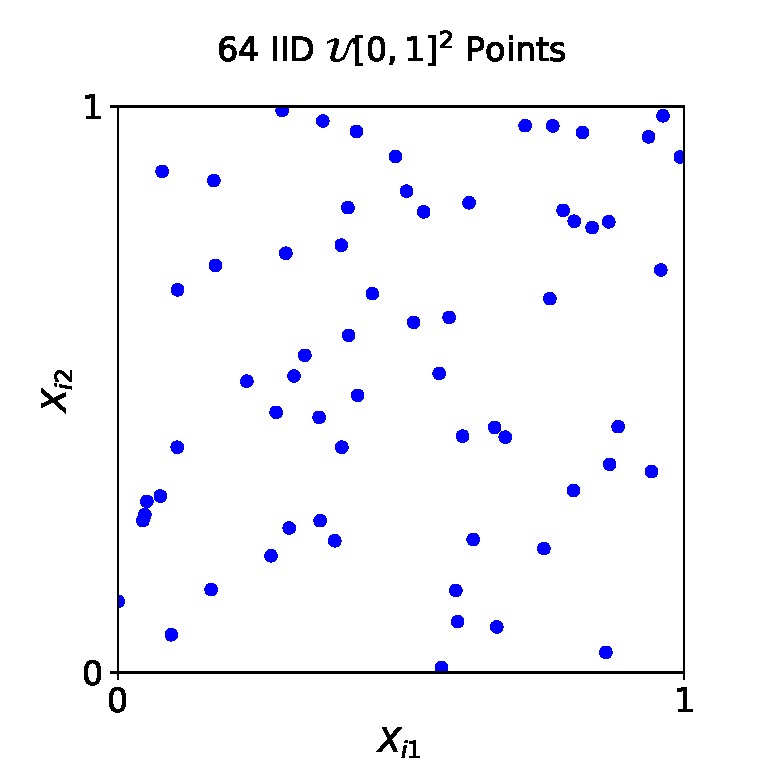
\includegraphics[height = 4.5cm]{ProgramsImages/iid_scatter.eps} \quad
	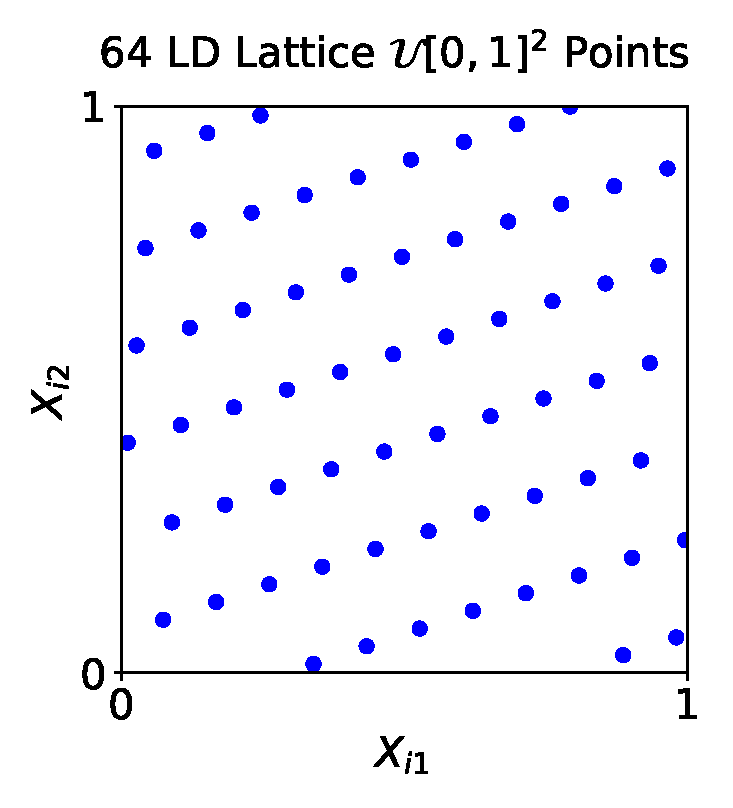
\includegraphics[height = 4.5cm]{ProgramsImages/lattice_scatter.eps} \quad
	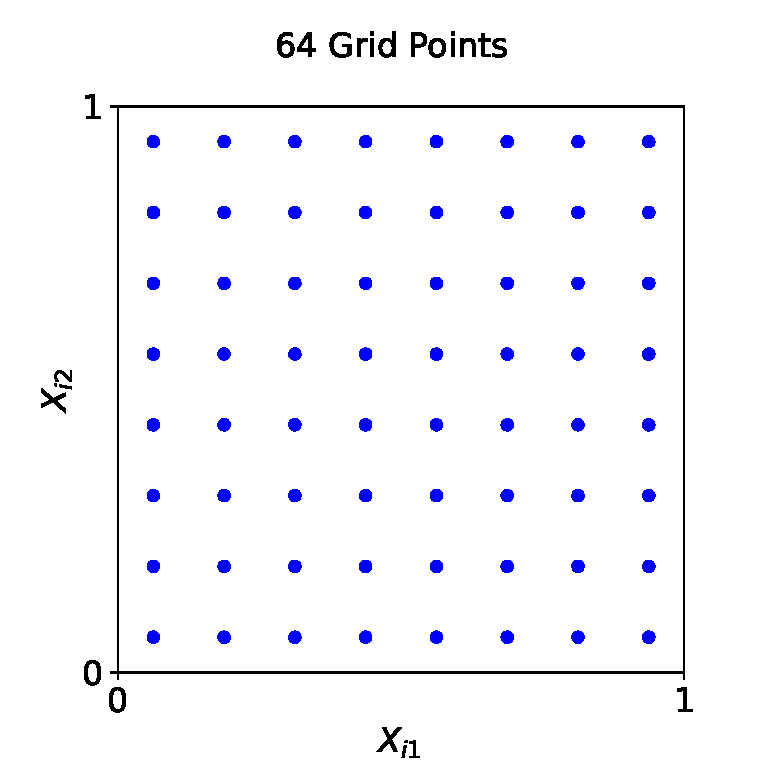
\includegraphics[height = 4.5cm]{ProgramsImages/grid_scatter.eps}
	\caption{IID points (left), LD lattice points (center), and grid points (right).  The LD points have fewer gaps and clusters of points than either the IID or grid points. \label{fig:iid_vs_ld}}
\end{figure}

%%%%%%%%%%%%%%%%%%%%%%%%%%%%%%%%%%%%%%%%%%%%%%%%%
\subsection{Efficiency Benefits from LD Sampling} \label{sec:eff_benefits}
%%%%%%%%%%%%%%%%%%%%%%%%%%%%%%%%%%%%%%%%%%%%%%%%%
The root mean squared error of the sample mean, $\hmu_n$ when IID samples are used is
$\std(Y)/\sqrt{n}$, where $\std(Y) = \sqrt{\int_{\cube} \abs{f(\bx) - \mu}^2 \, \dif \bx}$.  The smoothness required of $f$ is minimal, and the error bound has no curse of dimensionality assuming that $\std(Y)$ does not explode with increasing dimension.  However, the convergence rate is a modest $\Order(n^{-1/2})$, which translates into a computational cost of $\Order(\varepsilon^{-2})$ to satisfy the error criterion
\begin{equation} \label{eq:error_crit}
	\abs{\mu -\hmu_n} \le \varepsilon.
\end{equation}


For LD sampling the absolute error has a deterministic  upper bound of \cite{Nie92,Hic99a}
\begin{equation} \label{eq:KH}
    \abs{\mu - \hmu_n} \le D(\{\bX_i\}_{i=1}^n) \norm[\calf]{f - \mu}.
\end{equation}
The Banach space $\calf$ requires somewhat more smoothness than the $L^2$ requirement for IID sampling, e.g., $L^2$ mixed partial derivatives of up to order one in each coordinate direction. The discrepancy,  $D(\{\bX_i\}_{i=1}^n)$, corresponds to the norm of the cubature error functional \cite{Hic97a}, and is typically $\Order(n^{-1 + \delta})$, where $\delta$ is arbitrarily small and positive. This faster convergence rate translates into a computational cost of $\Order(\varepsilon^{-1-\delta})$ to satisfy error criterion \eqref{eq:error_crit}.

Fig.\ \ref{fig:KeisterTimes} displays results from our QMCPy \cite{QMCPy2020a} for  a computational physics example of Keister \cite{Kei96},
\begin{equation} \label{eq:Keister}
\mu = \int_{\reals^d} \cos( \norm[2]{\bt}) \exp(-\norm[2]{\bt}^2) \, \dif \bt,
\end{equation}
for the case $d =5$, $\mu \approx 1.135$ under several absolute error tolerances, $\varepsilon$.  QMCPy increases $n$ until \eqref{eq:error_crit} is satisfied according to the suitable stopping criteria.
Both the number of function values and the computation time increase like $\Order(\varepsilon^{-2})$ for IID sampling and $\Order(\varepsilon^{-1-\delta})$ for LD sampling as $\varepsilon$ decreases. For $\varepsilon = 0.01$ there is a hundred-fold contrast between the $n$ and time required for IID versus LD. 

\begin{wrapfigure}{r}{0.63\textwidth}
	\centering
	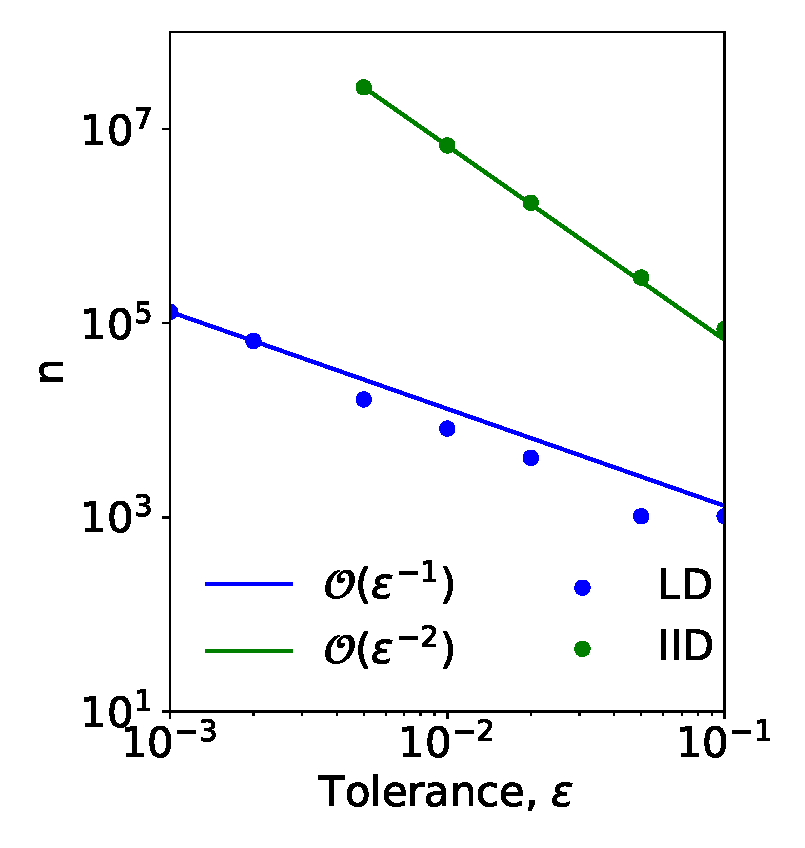
\includegraphics[height =0.32\textwidth]{ProgramsImages/keister_n.eps}
	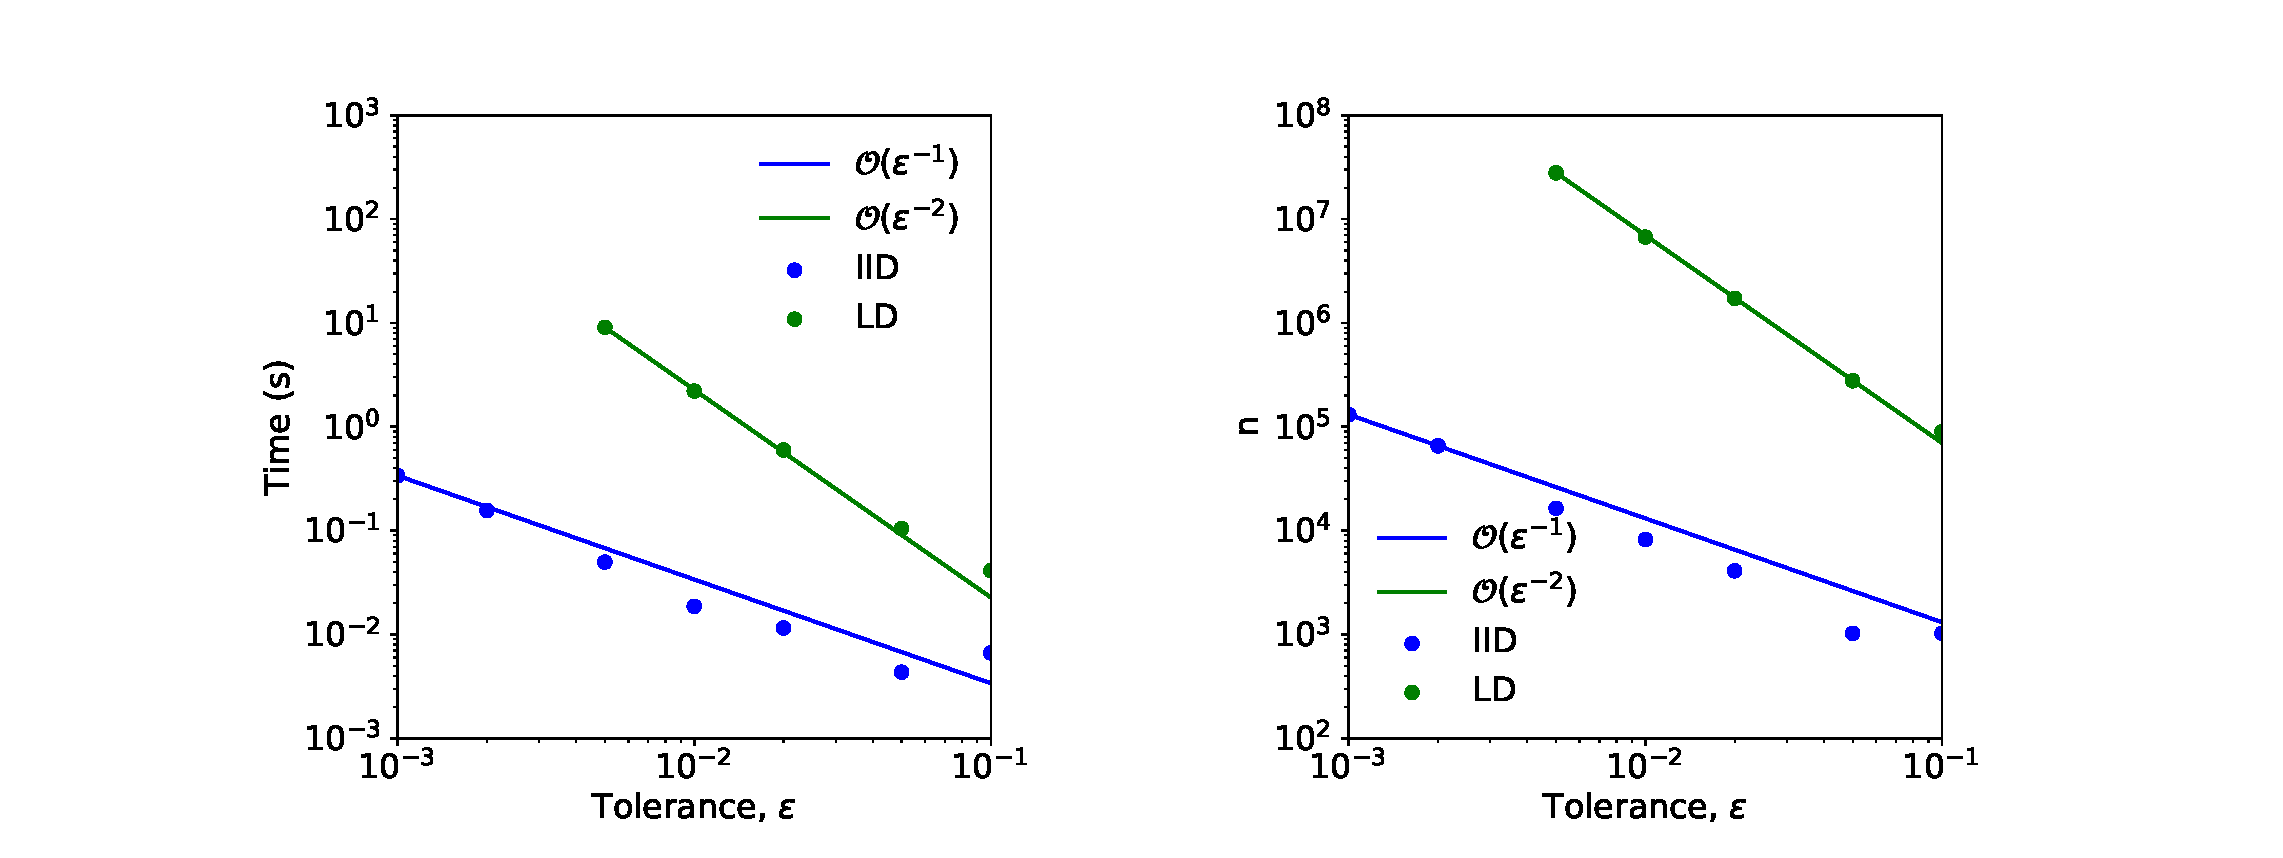
\includegraphics[height =0.32\textwidth]{ProgramsImages/keister_timing.eps}
	\caption{Number of function values (left) and run time (right) required to compute the Keister integral \eqref{eq:Keister} using QMCPy.  LD sampling is substantially more efficient than IID sampling, especially as the error tolerance decreases.}
	\label{fig:KeisterTimes}
\end{wrapfigure}



The orders of the computational cost dependence on $\varepsilon$ for IID and LD sampling are \emph{independent of $d$}.  This is not the case for tensor product rules and grid sampling.  If the derivatives of $f$ up to total order $rd$ exist, then tensor product rules may satisfy \eqref{eq:error_crit} at a computational cost of $\Order(\varepsilon^{-d/r})$.  Increased smoothness, $r$, helps but cannot overcome the exponential growth of the cost with $d$.

To harness the efficiency of LD sampling via QMC methods, practitioners need quality software that is easy to use.  QMC researchers need a showcase  for their latest work.  QMCPy satisfies that.

%%%%%%%%%%%%%%%%%%%%%%%%%%%%%%%%%%%%%%%%%%%%%%%%%
\section{QMCPy to Date}
%%%%%%%%%%%%%%%%%%%%%%%%%%%%%%%%%%%%%%%%%%%%%%%%%

%%%%%%%%%%%%%%%%%%%%%%%%%%%%%%%%%%%%%%%%%%%%%%%%%
\subsection{The Start of QMCPy}
%%%%%%%%%%%%%%%%%%%%%%%%%%%%%%%%%%%%%%%%%%%%%%%%%
The better existing QMC software packages include the following:
BRODA (Sobol' sequences) \cite{BRODA20a}, GAIL (automatic stopping criteria) by \FH, \SCTC and collaborators \cite{ChoEtal20a}, LatNet Builder (generators for lattices and digital nets) \cite{LatNet}, MATLAB (Sobol' and Halton sequences) \cite{MAT9.10}, Multi-Level (Quasi-)Monte Carlo routines  by Giles \cite{GilesSoft}, Magic Point Shop (lattices and Sobol' sequences) \cite{Nuy17a}, OpenTURNS \cite{OpenTURNS}, randomized Halton sequences by \AO \cite{Owe20a}, PyTorch (scrambled Sobol' sequences) \cite{paszke2019pytorch}, QMC4PDE (QMC for elliptic PDEs with random diffusion coefficients) \cite{KuoNuy16a}, QRNG (Sobol' and Halton sequences) \cite{QRNG2020}, LD Sequences by Robbe \cite{Rob20a}, SciPy \cite{virtanen2020scipy}, Stochastic Simulation in Java \cite{SSJ}, and
UQLab \cite{UQLab2014}.  These software packages are written in various languages.  
Each focuses on just certain aspects of QMC, such as the generation of LD sequences, fundamental QMC algorithms, or particular applications.  Whereas SciPy is a community effort, most of the other software packages are the efforts of individual research groups.

\MM's company, Silicon Valley startup SigOpt, now a part of Intel, offered to fund the early-stage development of  QMCPy in 2019. Python 3 was chosen as the language because of its popularity among a broad spectrum of potential users, especially those in the high-tech industry.  \AS,  at the time a co-terminal BS/MS student at Illinois Tech, and now an applied mathematics PhD student at Illinois Tech, was hired to create the QMCPy code.  QMCPy was released initially in the summer of 2020 and has had several upgrades since then.  QMCPy may be installed using \pyinline{pip} and imported via \pyinline{from qmcpy import *}.


%%%%%%%%%%%%%%%%%%%%%%%%%%%%%%%%%%%%%%%%%%%%%%%%%
\subsection{QMCPy Architecture}
%%%%%%%%%%%%%%%%%%%%%%%%%%%%%%%%%%%%%%%%%%%%%%%%%

The aforementioned discussions produced a skeleton for QMCPy consisting of four major abstract classes:
\begin{itemize}
	\item \pyinline{DiscreteDistribution} for generating LD and IID sequences,
	\item \pyinline{TrueMeasure} to accommodate more general distributions or measures,
	\item \pyinline{Integrand} to define the particular function, $f$, of interest, and
	\item \pyinline{StoppingCriterion} to determine when to stop the simulation.
\end{itemize}
An auxiliary class, \pyinline{AccumulateData}, keeps track of intermediate and final results.

\subsubsection{\textup{\pyinline{DiscreteDistribution} and \pyinline{TrueMeasure}}} LD sequences are constructed by creating the object and then generating points.  The code below produces the lattice points in the center panel of Fig.\ \ref{fig:iid_vs_ld}.
\begin{pythoncode}
ld = qmcpy.Lattice(dimension = 2)  #define a discrete LD distribution
points = lattice.gen_samples(n = 64)  #construct points
\end{pythoncode}

\begin{wrapfigure}{r}{0.65\textwidth}
	\centering
	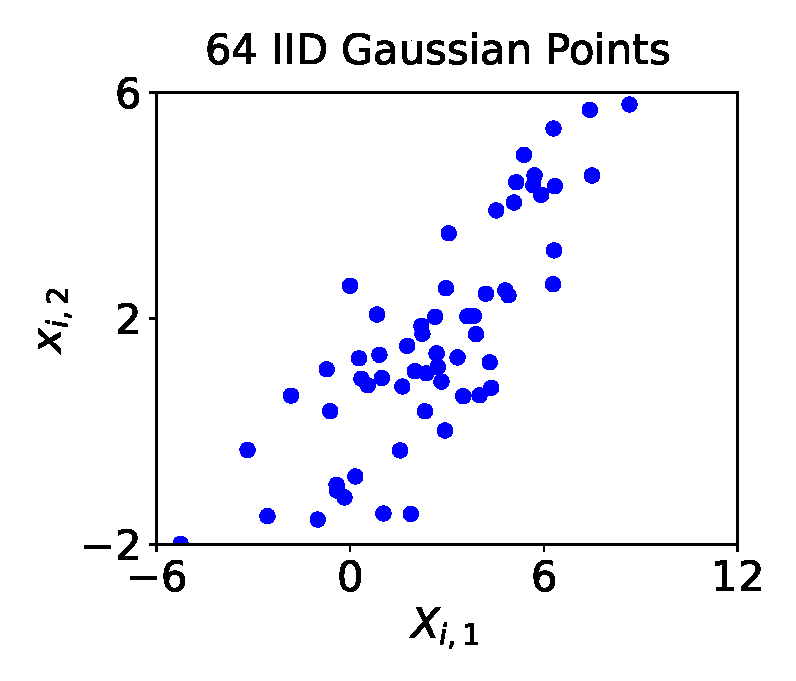
\includegraphics[height = 4.2cm]{ProgramsImages/Gauss_IID.eps}
	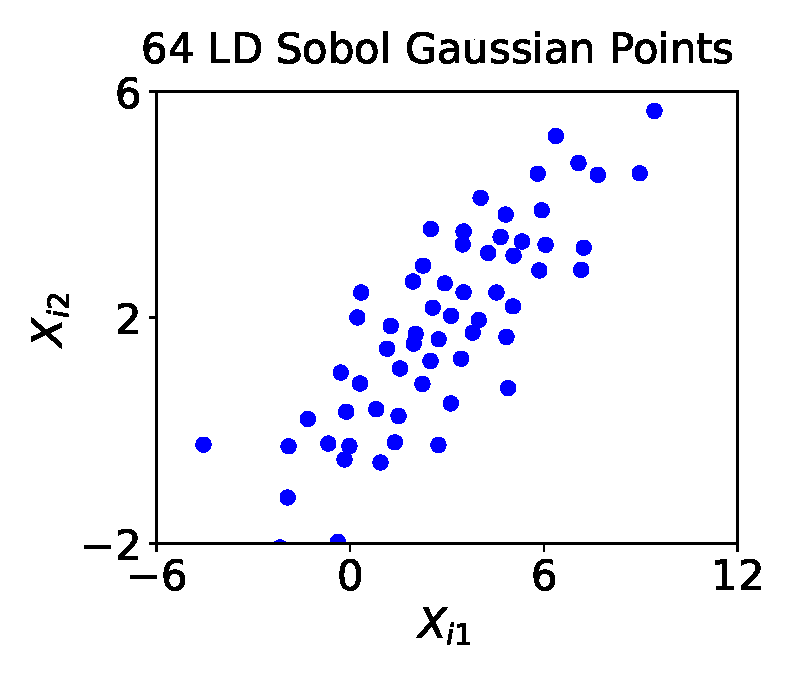
\includegraphics[height = 4.2cm]{ProgramsImages/Gauss_Sobol.eps}
	\caption{IID Gaussian (left) and Sobol'  points transformed to mimic a Gaussian distribution (right).  The LD points better represent the Gaussian distribution than the IID points. \label{fig:ld_Gauss}}
\end{wrapfigure}

LD generators provide points designed to mimic the distribution $\calu[0,1]^d$.  QMCPy also has \pyinline{Sobol} \cite{DicPil10a} and \pyinline{Halton} \cite{Hal60} LD generators whose syntax are comparable.
For comparison purposes, QMCPy  has standard uniform and normal psuedo-random generators adopted from \pyinline{numpy}.  Our LD generators are extensible;  one may generate additional points while reusing the original ones.   QMCPy LD generators are randomized by default to ensure that no points lie on the boundary of the unit cube and to improve the order of convergence of $\hmu_n$ to $\mu$ \cite{Owe97}.

The \pyinline{TrueMeasure} class automates the transformation required to construct good points that mimic distributions other than standard uniform.  The  inverse  distribution is often used.
\begin{pythoncode}
gaussian_ld = qmcpy.Gaussian(qmcpy.Lattice(2), mean = [3,2], covariance = [[9,5],[5,4]])  #specify the distribution parameters
points = gaussian_ld.gen_samples(n = 64)  #construct points
\end{pythoncode}

Fig.\ \ref{fig:ld_Gauss} displays  IID and Sobol' points  transformed to mimic the Gaussian distribution with mean $\begin{pmatrix} 3 \\ 2 \end{pmatrix}$ and covariance matrix $\begin{pmatrix} 9 & 5 \\ 5 & 4 \end{pmatrix}$.  Transformed low discrepancy points may or may not be low discrepancy with respect to the new distribution, depending on how one defines the discrepancy \cite{LiKanHic20a}.  But, transformed low discrepancy points often outperform IID points in Monte Carlo calculations.

%%%%%%%%%%%%%%%%%%%%%%%%%%%%%%%%%%%%%%%%%%%%%%%%%
\subsubsection{\textup{\pyinline{Integrand} and \pyinline{StoppingCriterion}}}
%%%%%%%%%%%%%%%%%%%%%%%%%%%%%%%%%%%%%%%%%%%%%%%%%
For computing expectations and multivariate integration as described in \eqref{eq:mean}, one must specify the integrand.  The original form of the problem may not be convenient for computation.  For example, the Keister integral in \eqref{eq:Keister} can be thought of as an integral of $g$ with respect to the Gaussian distribution with zero mean and covariance $\mI/2$:
\begin{multline} \label{eq:KeisterAlt}
\mu = \int_{\reals^d} \underbrace{\pi^{d/2} \cos( \norm[2]{\bt})}_{g(\bt)}  \, \underbrace{\pi^{-d/2}\exp(-\norm[2]{\bt}^2)\, \dif \bt}_{\caln(\bzero, \mI/2)}
= \int_{\reals^d} \underbrace{\cos( \norm[2]{\bt}) \exp(-\norm[2]{\bt}^2)}_{h(\bt)}  \, \underbrace{\dif \bt}_{\text{Lebesgue}} \\
=   \int_{[0,1]^d} f(\bx) \, \dif \bx \qquad \text{for an appropriate transformation } \bt = \bT(\bx).
\end{multline}
Alternatively, $\mu$ can be thought of as an integral of $h$ with respect to Lebesgue measure.  QMCPy can compute the integral either way.

The first way begins by constructing the Gaussian transformed LD \pyinline{TrueMeasure} instance \pyinline{gs} as discussed in the previous section.  Next, one defines the function $g$ as in \eqref{eq:KeisterAlt} above.   \pyinline{CustomFun}  constructs an $f$ for which the integral, $\mu$, can be written in terms of the uniform distribution, which the LD sequence mimics.   \pyinline{CustomFun} automatically constructs the transformation $\bT$ in \eqref{eq:KeisterAlt}.
\begin{pythoncode}
gs = qmcpy.Gaussian(qmcpy.Sobol(5), covariance = 1/2)    #choose the Gaussian distribution
def g(t):  #your desired integrand, calculations must be vectorized
	d = t.shape[1]
	g_val = np.pi**(d/2) * np.cos(np.sqrt((t**2).sum(1)))
	return g_val  #size n vector
f = qmcpy.CustomFun(gs, custom_fun = g)
sc = qmcpy.CubQMCSobolG(f, abs_tol = 1e-3)   #stopping criterion must match  points
solution = sc.integrate()
\end{pythoncode}

The final stage of the computation requires the construction of a \pyinline{StoppingCriterion} instance, \pyinline{sc}.  The one here is due to PI \FH and \hypertarget{LlAJRlink}{Llu\'is Antoni Jim\'enez Rugama} (\LlAJR) \cite{HicJim16a} and is based on Walsh transformations of the sampled integrand data.  Invoking the \pyinline{integrate} method of \pyinline{sc} yields $\hmu_n$ satisfying \eqref{eq:error_crit}.

Another way to compute the Keister integral, see \eqref{eq:KeisterAlt}, is to think of it as an integral with respect to the Lebesgue measure.  Again \pyinline{CustomFun} makes the proper variable transformation.  The answer returned by QMCPy is the same as the first way, but this second way takes about twice the time.  The choice of variable transformation, $\bT$ that defines the  integrand $f$ from the original integrand is equivalent to importance sampling.  Automatic and adaptive importance sampling requires further research (see Sec. \ref{sec:??}).

 %%%%%%%%%%%%%%%%%%%%%%%%%%%%%%%%%%%%%%%%%%%%%%%%%
 \subsection{QMCPy Options}
 %%%%%%%%%%%%%%%%%%%%%%%%%%%%%%%%%%%%%%%%%%%%%%%%%
 QMCPy has several options for users to choose:
 \begin{itemize}
 	\item \pyinline{backends} for \pyinline{Sobol} from  QRNG \cite{QRNG2020},  SciPy \cite{virtanen2020scipy}, and MPS \cite{Nuy17a};

 	\item \pyinline{backends} for \pyinline{Lattice} from GAIL \cite{ChoEtal20a} and MPS \cite{Nuy17a}, and generators  from LatNet Builder \cite{LatNet};

 	\item \pyinline{StoppingCriteria} based on the \hypertarget{CLTlink}{Central Limit Theorem} (\CLT) for IID sampling and random replications of LD sampling;  a more rigorous criterion for IID sampling based on a Berry-Essen inequality \cite{HicEtal14a};  criteria for LD sampling based on fast transforms of integrand data \cite{HicJim16a, JimHic16a,RatHic19a}; most of these have arisen from the NSF-supported research of \FH, \SCTC and their collaborators, \AO, \hypertarget{LJlink}{Lan Jiang} (\LJ),
 	\LlAJR, \hypertarget{JRlink}{Jagadeeswaran Rathinavel} (\JR), and implemented in GAIL \cite{ChoEtal20a}.

 	\item Specification of relative error tolerances as well as absolute error tolerances;

 	\item Multi-level Monte Carlo methods; and

 	\item A few use cases, i.e., pre-programmed \pyinline{Integrand} instances.
 \end{itemize}

%%%%%%%%%%%%%%%%%%%%%%%%%%%%%%%%%%%%%%%%%%%%%%%%%
\subsection{QMCPy Support}
%%%%%%%%%%%%%%%%%%%%%%%%%%%%%%%%%%%%%%%%%%%%%%%%%
QMCPy is hosted on GitHub \cite{QMCPy2020a}. Bugs can be reported and features requested on the issues page.  Pull requests can be made by those who wish to add features.  All features are documented \cite{QMCPyDocs} using ReadtheDocs.  Doctests ensure that features work as expected. Features are illustrated by Jupyter notebooks.  \FH gave a tutorial on QMC software---with a focus on QMCPy---at MCQMC 2020 \cite{MCQMC2020QMCPyTut}.  A Google Colaboratory Notebook \cite{QMCPyTutColab2020} is available so that those watching  can try out QMCPy themselves in real time.  \FH, \SCTC, \AO, \AS \MM, and \PR wrote a series of blogs \cite{QMCBlog} to introduce QMC to the broader community of QMC.

%%%%%%%%%%%%%%%%%%%%%%%%%%%%%%%%%%%%%%%%%%%%%%%%%
\section{QMCPy in the Future}
%%%%%%%%%%%%%%%%%%%%%%%%%%%%%%%%%%%%%%%%%%%%%%%%%
QMCPy has made a good start.  Yet, much must be done to establish the critical mass of algorithms and collaborators that will make QMCPy  self-sustaining.  QMC theory is over 60 years old, yet there are also several methodological and theoretical issues to be addressed, especially to expand the scope of applicability of QMC.   The subsections below highlight those research problems that we will tackle.  We indicate the primary investigators and collaborators who will be addressing these problems and the time periods over which they will be addressed.


%%%%%%%%%%%%%%%%%%%%%%%%%%%%%%%%%%%%%%%%%%%%%%%%%
\subsection{Performance} [\FH lead, \AS, \DN, \AO{}] \label{sec:performance}
%%%%%%%%%%%%%%%%%%%%%%%%%%%%%%%%%%%%%%%%%%%%%%%%%


%%%%%%%%%%%%%%%%%%%%%%%%%%%%%%%%%%%%%%%%%%%%%%%%%
\subsubsection{Richer LD Sequence Generators } [Years 1--2] \label{sec:richLD}
%%%%%%%%%%%%%%%%%%%%%%%%%%%%%%%%%%%%%%%%%%%%%%%%%
Although QMCPy already includes the most popular LD sequences, we will implement more flexibility.  We will expand our generators to include \emph{higher-order digital sequences} \cite{Dic09a, Dic11a}, which yield  faster convergence rates  $n \to \infty$ for smooth integrands, such as those arising in computing multivariate probabilities.  Higher-order nets are not yet available in popular libraries.

For flexibility, the random digital scrambling and shifting of digital nets will be implemented so that either one or both can be turned on or off.  Linear matrix scrambling (LMS) \cite{Mat98,HonHic00a} is the simpler and more common method for randomizing digital sequences (such as the Sobol' sequence).  The original nested uniform scrambling (NUS) proposed by \AO \cite{Owe95} requires more complex code and a longer computation time, but it has a \CLT  \cite{Loh01}.  We will \emph{implement NUS} in QMCPy.

Implementing a richer class of LD sequence generators combined with QMCPy's growing set of use cases will allow us to test which LD sequence generators perform better in practice, e.g., Niederreiter vs.\ Sobol' or LMS vs.\ NUS. If we detect that certain sequences or some scrambling methods substantially outperform in practice, then we will develop a \emph{theoretical description} of when that happens.

%%%%%%%%%%%%%%%%%%%%%%%%%%%%%%%%%%%%%%%%%%%%%%%%%
\subsubsection{Speed-Up}
%%%%%%%%%%%%%%%%%%%%%%%%%%%%%%%%%%%%%%%%%%%%%%%%%
Python's advantages are ease of coding and the rapidly growing code base.  However, Python code does not execute particularly quickly.  Python can be made to execute more quickly by re-writing it in C or utilizing GPUs.  For example, this is done for some of the PyTorch code and the TensorFlow code.  We will speed up critical QMCPy code by \emph{re-writing it in C}.

There have been attempts at parallel implementations of LD sequences \cite{LiMul00a,OktSri02, SchUhl01,WanEtal06a,LiuHic04a}, but there is no generally accepted parallel LD software library.  There are issues with load balancing.  Does one give different processors different segments of the same LD sequence?  Or does one combine the results of several randomized LD sequences, each from a different processor?

We will \emph{implement LD sequences taking advantage of multiple cores} of the same CPU.  We will also explore the possibility of GPU implementations.  Python parallel computing resources \cite{ParallelPython}, such as Numba \cite{Numba} will prove invaluable.


\subsection{Theoretical Issues Surrounding Discrepancy and Convergence} [\FH lead, \AS]
The discrepancy in \eqref{eq:KH} measures the difference between the empirical distribution of the sampling sites and the uniform distribution.  When the original integral is defined with respect to a different distribution, as in \eqref{eq:KeisterAlt}, we must perform a variable transformation:
\begin{equation}\label{eq:imp}
	\mu = \int_{\reals^d} g(\bt)  \, \dif F(\bt)
	=   \int_{[0,1]^d} f_{\bT}(\bx) \, \dif \bx \qquad \text{for an appropriate transformation } \bt = \bT(\bx).
\end{equation}

A perspective is that we transform our sampling points to mimic the original distribution, $F$, and work with  the error bound derived by \FH in \cite{Hic99a}:
\begin{equation}
	\abs{ \mu  - \frac 1n \sum_{i=1}^n g(\bT(\bX_i))} \le  D(\{\bT(\bX_i)\}_{i=1}^n,F ) \norm[\calg]{g - \mu},
\end{equation}
where the discrepancy $D(\{\bT(\bX_i)\}_{i=1}^n,F )$ is a distance between the empirical distribution of the transformed points and the distribution defining the integral.    This discrepancy is defined in terms of the reproducing kernel, $K$, for the Hilbert space $\calg$.  The advantage of this approach is that it may be easier to determine whether $g- \mu$ has a small $\calg$-norm than determine whether $f_\bT-\mu$ has a small $\calf$-norm.

There is no theory to say under what conditions small  $D(\{\bX_i\}_{i=1}^n)$ implies small  $D(\{\bT(\bX_i)\}_{i=1}^n,F )$.  Indeed our recent study \cite{LiKanHic20a} suggests that this is not always the case.  We will derive conditions under which the transformation of low discrepancy points yields low discrepancy points.  This will involve assumptions on the reproducing kernel $K$ and the distribution $F$.

\FJHNote{Strong law of large numbers for lattices}


\subsection{Variance/Variation Reduction Through Importance Sampling and Control Variates} [\FH lead]
The QMC error bound in \eqref{eq:KH} contains the factor $\norm[\calf]{f - \mu}$, which may be called the \emph{variation} of the integrand.  For randomized QMC, the mean squared error of $\hmu_n$ is its variance.  Substantial error reduction can sometimes be obtained by rewriting the integral to reduce the variation or variance.  Examples include rare event modeling \cite{rubino2009rare} and Bayesian inference \cite{salmeron2000importance}.

Importance sampling \cite{owen2000safe} is a variance/variation reduction tool whereby one samples from a new distribution (the \textit{importance} distribution) to place greater weight where the integrand varies more. Since LD sampling at its heart is $\calu[0,1]^d$, LD sampling to mimic a different distribution can be thought of as choosing a variable transformation, $\bT$ in \eqref{eq:imp}.
Since $\bT$ is not unique---as shown in the Keister example \eqref{eq:KeisterAlt}---the challenge lies in finding a good choice for $\bT$ that makes the variation, $\norm[\calf]{f_{\bT} - \mu}$, small. Key developments include the annealed importance sampler \cite{neal2001annealed}, the bridge sampler \cite{gelman1998simulating}, and \AO's safe importance sampler \cite{owen2000safe}. Recent work includes \cite{mueller2019neural}, which uses deep neural networks for importance sampling in image rendering, and \cite{huling2020energy}, where PI \SM extends importance sampling for covariate balancing in causal inference.

Control variates or de-trending \cite{Gla03} is another powerful variance/variation reduction technique. The idea is to obtain a new integrand, $\tilde{f}$, by subtracting from the original integrand a linear combination of functions (control variates) whose integrals are zero.  If $\tilde{f}$ has smaller variation/variance than the original integrand, $f$, then substantial cost savings are possible.  Control variates are widely used in financial pricing and stochastic simulations. Important works (among many) include \cite{nelson1990control}, which investigates control variate remedies, and the QMC control variates papers \cite{HicEtal03, Hic17a} by \AO, PI \FH, and collaborators. Recently, \cite{mueller20neural} introduced the neural control variates method, which uses a neural network to learn an optimal choice of control variate for variance reduction.

\textit{We will implement these variance/variation reduction methods} in QMCPy and attempt to automate the choices of transformation and control variates. This will provide  a comprehensive and accessible toolbox of variance reduction methods for a broad range of applications. \FJHNote{Theory?}

\subsection{Multilevel QMC (MLQMC)}[\SM lead]
For high or infinite dimensional integration problems, the computational cost of the integrand is often proportional to $d$, which makes the cost of the sample mean $\Order(dn)$.  Multilevel (Q)MC \cite{Gil15a} decomposes the original integral into a sum of several integrals with different numbers of variables, $d_1 < \dots < d_L$.  The total cost is then $\Order(d_1 n_1 + \cdots + d_L n_L)$. When done well, error criterion \eqref{eq:error_crit} can be met for a decreasing sequence $n_1 > \dots > n_L$, which results in an overall large cost savings compared to a single level (Q)MC algorithm requiring $\Order(d_Ln_1)$ operations. \emph{We will strengthen} QMCPy's rudimentary MLQMC, including extending the theory and implementation of the single level stopping criteria developed by PI \FH, \SCTC, and their collaborators \cite{HicEtal14a,HicJim16a,JimHic16a,HicEtal17a,RatHic19a} to the multilevel case.

An urgently-needed yet relatively unexplored area is the use of QMC as design points for multi-level functional approximation. These approximations are widely-used as efficient surrogate models for expensive scientific computations, which can be used for scientific investigation and decision-making in a timely manner (the PI \SM has ...). \SMNote{Add related work from Karen Willcox and Max Gunzburger} \SMNote{We have a nearly-finished paper applying multilevel QMC points as designs for multi-fidelity emulators. I can add in some preliminary results on this. Arc-sin \& experimental design. Dispersion scales terribly in dimension.}

\iffalse
\subsection{Density Estimation}

Much of the QMC literature focuses on estimating the population \textit{mean}, $\mathbb{E}(Y)$. In many problems, however, one may be interested in estimating the underlying probability \textit{density} of $Y = f(\bX)$. The state-of-the-art in the classical setting, is kernel density estimation \cite{silverman1986density}, which uses IID samples $Y_1, \dots, Y_n$ to approximate $\varrho$ by:
\begin{equation}\label{eq:kerndens}
\hat{\varrho}_n(y) = \frac{1}{n} \sum_{i=1}^n \frac{1}{h} \fK \left( \frac{y - Y_i}{h} \right),
\end{equation}
where $\fK$ is a symmetric kernel, and $h>0$ is the bandwidth parameter.

Given the improvement that QMC gives for mean estimation, a natural question is whether QMC also provides gains for density estimation. A recent paper \cite{abdellah2018density} by \AO and coauthors explores this by replacing the IID samples $\{\bX_i\}_{i=1}^n$ used to generate $Y_i = f(\bX_i)$ with randomized LD samples \cite{owen2000monte}. They showed that this new QMC density estimator enjoys an improved rate of convergence over the standard estimator \eqref{eq:kerndens}, both theoretically and in numerical experiments.

\textit{We will implement this QMC kernel density estimation method} in QMCPy. This will provide users from a broad range of fields, from engineers to data scientists, a useful tool for accurate density estimation when sample data is limited or expensive to collect.

\fi

% \subsubsection{Uncertainty Propagation}

% \iffalse
% Pierre L'Ecuyer's talk
% https://media.ed.ac.uk/playlist/dedicated/51612401/1_0z0wec2z/1_r1x3xmle

% https://drive.google.com/file/d/1uztn18UimvdIo3hyYXywUaOxj_wqPJ7N/edit

% \fi

% MLQMC
%\end{document}

\iffalse
\subsubsection{Sobol' Indices} In sensitivity analysis, Sobol' indices, which are defined as multidimensional integrals, play an important role.  We will implement the work done by \LlAJR and others \cite{GilEtal16a,GilJim16b} to adaptively compute Sobol' indices.  \AO will encourage his PhD student, Chris Hoyt, to help.
\fi

\subsection{Big Data Analytics} [\SM lead] Big data is ubiquitous with recent advances in experimental technology and computing power.  A key challenge is making use of this rich source of data; learning algorithms need to be highly \textit{efficient} and \textit{scalable} to extract information for real-time decision-making. This development is an important research direction in statistics and computer science.

One way to make these algorithms scalable is to iteratively train the model on small batches of the data, typically sampled uniformly at random. This is widely used to scale up many powerful machine learning algorithms, such as stochastic gradient descent (SGD, \cite{Bot2010}) and stochastic gradient boosting \cite{friedman2002stochastic}. Consider SGD as an example. The objective is to minimize the loss $L(\theta;\mathcal{X}) = N^{-1} \sum_{m=1}^N l(\theta;\bX_m)$ over model parameters $\theta \in \mathbb{R}^q$, where $\mathcal{X} = \{\bX_m\}_{m=1}^N \subset \mathbb{R}^d$ is the large training data. Standard gradient descent methods for optimization \cite{nocedal2006numerical} are impractical here, since they require evaluation of the full gradient $N^{-1} \sum_{m=1}^N \nabla l(\theta;\bX_m)$, which is very expensive for big data. Mini-batch SGD \cite{Bot2010} approximates this gradient using a subsample $\mathcal{X}_{s}^{[l]} \subset \mathcal{X}$ of size $n \ll N$, taken IID and uniformly from the big data $\mathcal{X}$. The descent steps are then iterated until convergence:
\begin{equation}\label{eq:sgdopt}
\theta^{[l+1]} \leftarrow \theta^{[l]} - \eta \left( \frac{1}{n} \sum_{\bX \in \mathcal{X}_{s}^{[l]}} l(\theta;\bX)\right) , \quad l = 1, 2, \cdots,
\end{equation}
where $\eta$ is the gradient descent step size. Mini-batch SGD is widely used for scalable training of neural networks and deep learning models with big data \citep{srivastava2014dropout}.

SGD has a notable limitation: since its gradients are estimated by random subsampling, the solution sequence $(\theta^{[l]})_{l=1}^\infty$ converges to a \textit{noise ball} of radius $\mathcal{O}(n^{-1})$ around the global optimum $\theta^*$. For small subsample sizes $n$, SGD can therefore return parameter estimates very far from  $\theta^*$. One solution is to carefully choose a small LD dataset that well-represents the big data $\mathcal{X}$. This is referred to as ``data squashing'' \cite{owen2003data} by \AO, and has garnered attention in recent years (see, e.g., leverage-score subsampling \cite{ma2015statistical}, coresets \cite{chan2006faster,bachem2017practical, huggins2016coresets}, and also recent work by the PI \SM \cite{mak2018support,mak2018minimax,mak2017projected,krishna2019distributional}). These methods, however, do not apply directly for the problem of data squashing for the target problem of stochastic (SGD) optimization.

We propose a new ``data squashing'' method which makes use of a LD subset of big data $\mathcal{X}$ for accelerating SGD optimization. The following preliminary \textit{theoretical} result guarantees the \textit{existence} of such a LD subset:
\begin{theorem}
Let $\mathcal{X} = \{\bX_m\}_{m=1}^N$ be any set of points on $[0,1]^d$. Suppose $n \leq \sqrt{N}$. Then there exists a subset $\mathcal{X}_s \subseteq \mathcal{X}$ of size $n$ which, when used within the SGD optimization iteration \eqref{eq:sgdopt}, yields a solution sequence $(\theta^{[l]})_{l=1}^\infty$ which converges to a noise ball of radius $\mathcal{O}\{(\log n)^{3d+1}/n^2\}$.
\end{theorem}

\SMNote{
\begin{itemize}
\item Discussion of theorem: rate improvement, condition for data, bound on $\mathcal{X}$, implications for optimization.
\item Task: solving for this LD subset, nonlinear FFT, evaluation time independent of $N$.
\end{itemize}
}
% \textit{We will implement these existing methods} in QMCPy, and explore their effectiveness in a suite of big data problems. There is little work on which data squashing procedure is most appropriate for SGD optimization. Our preliminary results show that a LD subsample exists for \textit{any} big dataset $\mathcal{X} \subset \mathbb{R}^d$ that achieves a noise ball radius of $\mathcal{O}\{(\log n)^{3d+1}/n^2\}$. We will investigate this further and implement this in QMCPy.

\subsection{Posterior Sampling for Complex Bayesian Models} [\SM lead]

\SMNote{Add motivation \& methodology \& preliminary results on randomized Stein points. Idea is to provide probabilistic inference for deterministic Bayesian sampling methods.} Bayesian methods have become quite popular in recent decades, primarily due to their ability to fit complicated models via sampling \cite{GelEtal13}. Such methods have largely relied on MCMC sampling for exploration of the posterior distribution $F$, which captures information on model parameters. However, with the rise of big data and complex machine learning models, the posterior distribution $F$ can be expensive to evaluate, which makes MCMC sampling very time-consuming \cite{joseph2015sequential}. This is compounded by the highly correlated nature of MCMC samples, which reduces the information provided by each sample \citep{link2012thinning}. For such problems, a LD posterior sampling method can greatly improve model learning given a time budget.

% While the QMC Metropolis method by \cite{OweTri05a} speeds up the convergence of samples, it still requires many posterior evaluations. We want method which can provide LD sampling with limited posterior evaluations here.

One approach for LD posterior sampling is to minimize the kernel discrepancy $D(\{\bX_i\}_{i=1}^n, F)$ in \eqref{eq:KH} for samples $\{\bX_i\}_{i=1}^n$. This is known as \textit{kernel herding} \citep{chen2012super}. Kernel herding has a key weakness for posterior sampling: the discrepancy, $D(\{\bX_i\}_{i=1}^n, F)$, to be optimized requires an analytic expression for the integral $\int K(t,\bX_i) \, \dif F(t)$ (see \eqref{eq:KHterms}), which is unattainable for complex posteriors $F$. To address this, \cite{chen2018stein} proposes a new \textit{Stein reproducing kernel} for discrepancy minimization:
\begin{multline}\label{eq:stein}
K_{st}(\bt,\bx) = \nabla_\bt \cdot \nabla_\bx K(\bt,\bx) + \nabla_\bt K(\bt,\bx) \cdot \nabla_\bx \log \dif F(\bx)\\
 + \nabla_\bx K(\bt,\bx) \nabla_\bt \log \dif F(\bt) + K(\bt,\bx) \nabla_\bt \log \dif F(\bt) \cdot \nabla_\bx \log \dif F(\bx),
\end{multline}
where $K$ is a symmetric, positive definite kernel, and $\nabla$ and $\nabla \cdot$ are the gradient and divergence operators. The key advantage is that the integral in question $\int K_{st}(t,\bX) \, \dif F(t)$ evaluates to 0 for all $\bX$, which allows one to generate LD posterior samples via minimization of discrepancy $D(\{\bX_i\}_{i=1}^n, F)$. This is a promising method that speeds up the learning of complex Bayesian models. \SMNote{specify problem carefully: expensive function evaluations? etc.}

\SMNote{expand on novel developments} \textit{We will implement Stein points} in QMCPy. PI \SM has worked on a variety of complex Bayesian modeling problems, from climatology \cite{mak2016regional} to aerospace engineering \cite{mak2018efficient,chang2019kernel,yeh2018common}, and we will explore the effectiveness of Stein points for such problems. We will also explore further extensions of Stein points for approximate Bayesian computation, a popular class of Bayesian methods for population genetics and epidemiology.

\iffalse
https://media.ed.ac.uk/playlist/dedicated/51612401/1_0z0wec2z/1_jkdkrau0

https://drive.google.com/file/d/1UfZinskltBhhAQcYFAzf26FIPFje5aM-/edit

\fi

\iffalse
\subsection{Uncertainty Quantification}
Uncertainty quantification is the science of quantifying, characterizing, tracing, and managing uncertainty in computational and real worlds systems \cite{smartuq, Smi14a}. Since data from such systems are typically expensive to simulate or collect, a key focus in this area is the sampling design for data collection, which can greatly benefit from QMC methods.

A recent application of QMC for uncertainty quantification is to compute the expectation of a functional of solution of a partial differential equation with random coefficients \cite{HerSch20a}. This has broad applications in engineering problems, e.g., fluid flow through a porous medium. QMCPy will implement a typical use case, which may show how to link QMCPy code with a PDE solver from another package. The PI \SM has done extensive work on uncertainty quantification, for rocket engine design \cite{li2017two,li2018uncertainty,chang2019kernel,yeh2018common,mak2018efficient}, neuroscience modeling \cite{wang2020uncertainty}, and active learning \cite{mak2018maximum}. We will explore the performance of LD sampling for these applications.
\fi

\iffalse 
\subsubsection{Ray Tracing}
Image rendering is a visually stunning application of QMC \cite{Keller2013a}.  QMCPy will implement a simple example to showcase the advantage of LD over IID sampling.
\fi

\subsection{Probabilistic Numerics (PN)}\hypertarget{PNlink}{} \FJHNote{Move to Section 4}
\PN assumes that the input function or solution of a mathematical problem is an instance of a random process.  This allows one to apply a probabilistic approach to construct credible intervals for the solution. PI \FH along with his former PhD student \JR developed a fast Bayesian cubature method \cite{RatHic19a} using lattice LD sampling.  Our collaborator \TS is a \PN expert.

Bayesian optimization applies this \PN perspective to finding the minimum of an objective function.  The next locations to sample the objective function are chosen as the optimum of an acquisition function, which in the Bayesian context takes the form of a $d$-variate integral, where $d$ is the number of future points to be sampled times the dimension of those points.  \MM illustrates the advantages of LD sampling for computing an acquisition function in his blog \cite[qEI with QMCPy]{QMCBlog}.  The observed function values are noisy.  As in the Keister example in Sect.\ \ref{sec:eff_benefits}, LD sampling shows a substantial advantage over IID sampling.

\begin{figure}[h]
	\centering
	%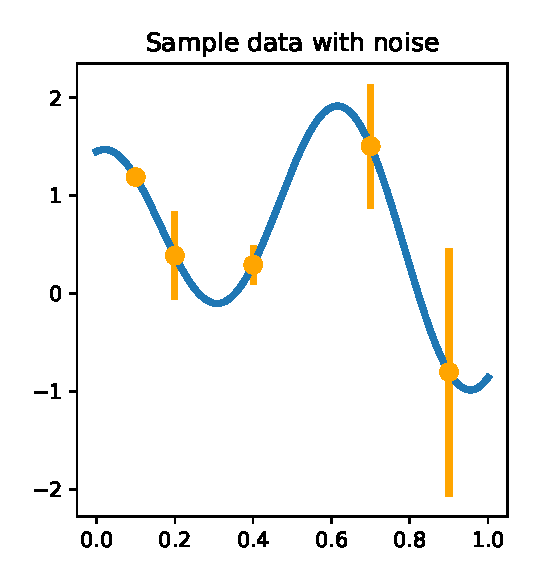
\includegraphics[height = 5cm]{ProgramsImages/sample_data.eps} \quad
	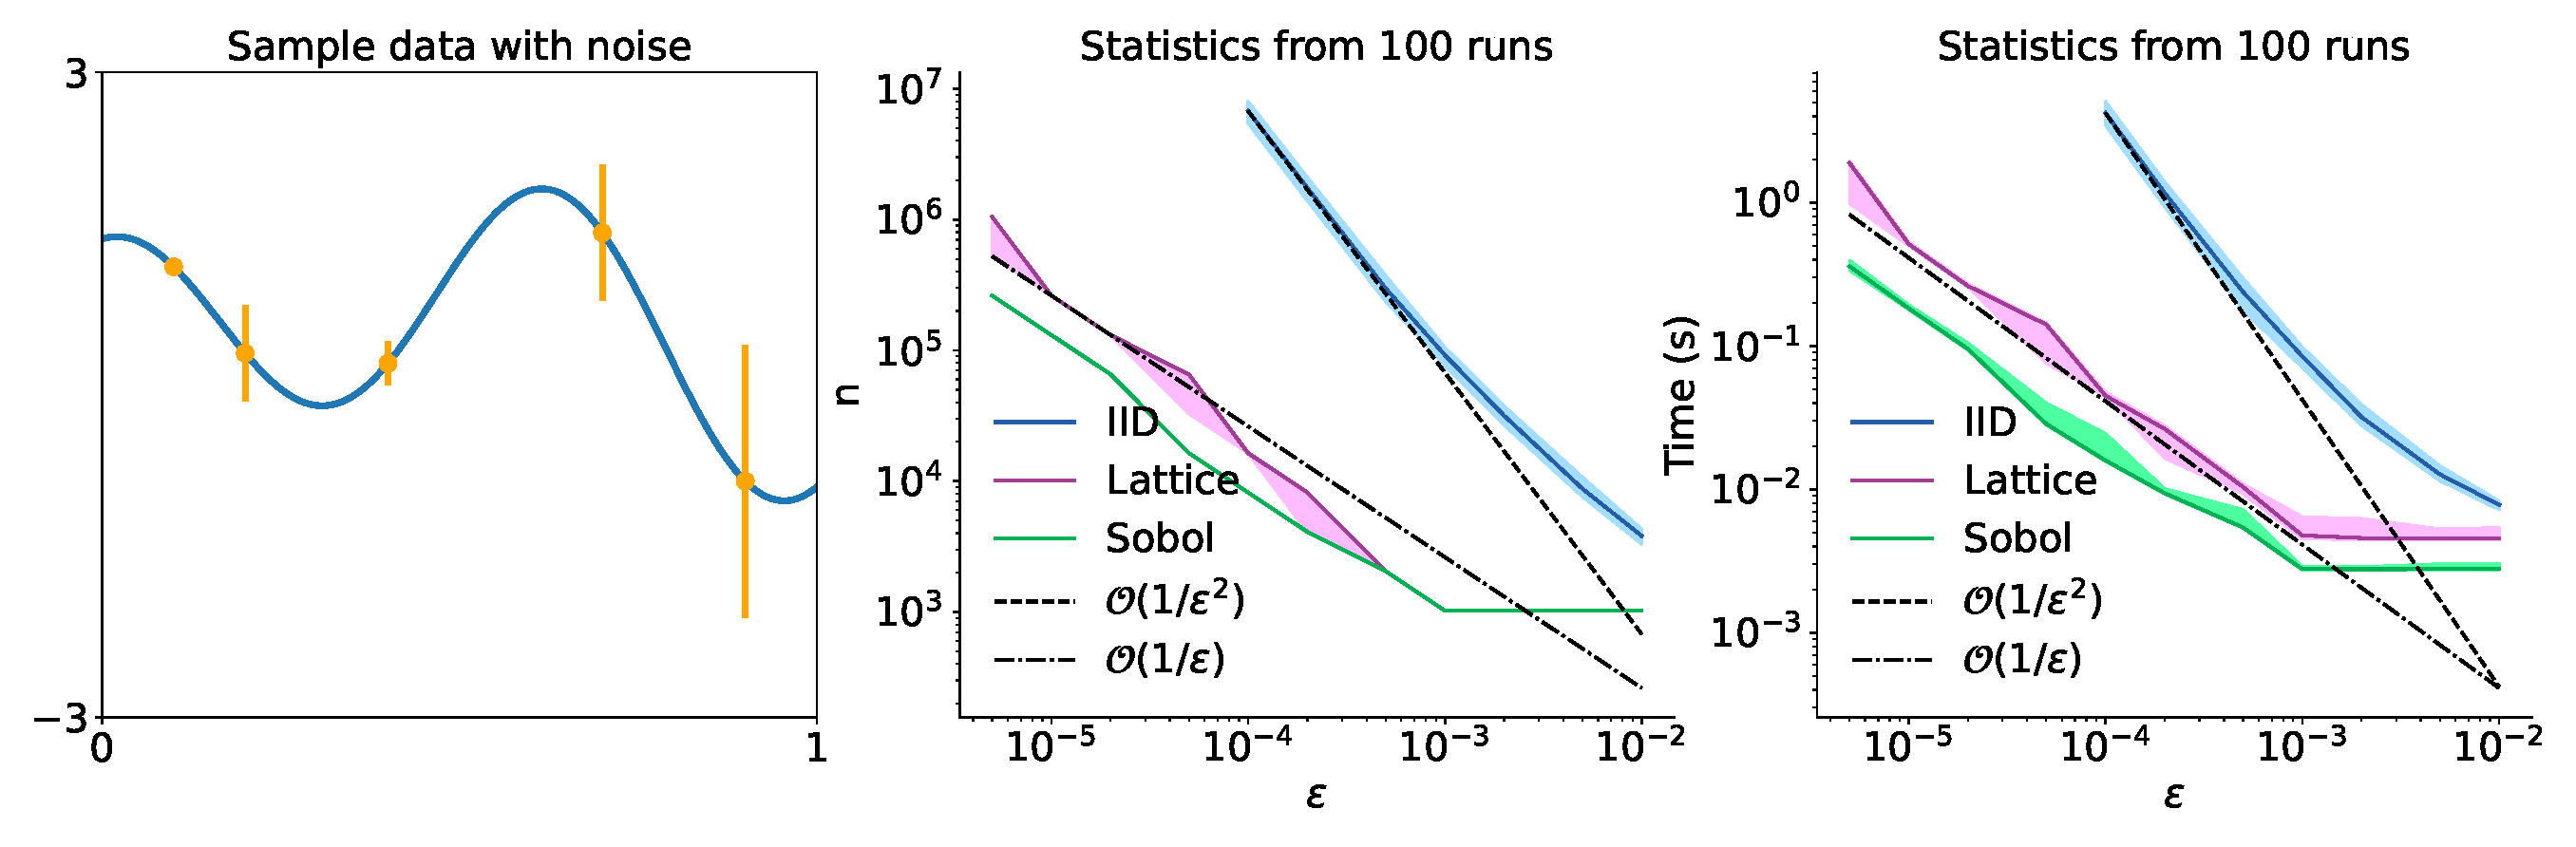
\includegraphics[height = 5cm]{ProgramsImages/qEI_cost_comp_time.eps}
	%
\includegraphics[height = 5cm]{ProgramsImages/qEI_cost_comp_n.eps}
	\caption{A one-dimensional objective function (left) and the number of function values (center) and run time (right), required to compute the acquisition function in \cite[qEI with QMCPy]{QMCBlog} to the desired tolerance, $\varepsilon$.  LD sampling is much more efficient than IID sampling, especially as the error tolerance decreases.}
	\label{fig:qei}
\end{figure}

Bayesian optimization is a relatively unexplored QMC application area. PI \SM has worked on black-box optimization \cite{mak2019analysis,chen2019hierarchical}, most notably on a hierarchical Bayesian optimization method \cite{chen2019hierarchical}. We will explore the \emph{efficacy of LD sampling} in Bayesian optimization and other \PN problems. \SMNote{new methodology \& theory: embedded Bayesian optimization?}






\section{Broader Impacts}

QMCPy will aggregate the best QMC software with a clear structure and a consistent user interface.  When a potentially better or interesting LD generator, algorithm, or use case arises, it will be a simple matter to swap out the old for the new and measure the performance while all other pieces remain the same.  Some compe \SCTCNote{Incomplete sentence}

\subsection{QMCPy as a Proving Ground}
QMCPy will \emph{stand in the breach} between research code from individual groups and large-scale software packages.  Research groups need to compare their new ideas with the best available.  Those who develop LD generators need to test them on a variety of use cases and as key components of various QMC algorithms.  Those with new QMC algorithms need to test them with the best generators.  Those with juicy use cases want to try the best that QMC offers.  Because large-scale software packages like \pyinline{scipy} or MATLAB, do not offer QMCPy's options,  QMCPy \emph{will attract a significant number of QMC researchers as contributors.}

Although large-scale software packages cannot adopt every new QMCPy wrinkle, QMCPy algorithms attracting broad interest can be folded into these large-scale packages. FH had this experience when MATLAB adopted his TOMS LD generators from \cite{HonHic00a}.

By making QMC methods easily accessible, QMCPy will \emph{introduce new application areas} to the benefits of LD sampling.  This will lead to \emph{LD sampling being incorporated} into the software packages used by practitioners in those disciplines. This includes, e.g., PyMC3 \citep{salvatier2016probabilistic} and PyStan \citep{stan2017pystan}, which are popular Python packages for Bayesian statistical modeling and probabilistic machine learning. \SMNote{added discussion on applications} The accessibility of state-of-the-art QMC methods will also spur on novel advancements in a diverse range of important disciplines, including machine learning, uncertainty quantification, causal analysis, Bayesian modeling, and sensitivity analysis. The PIs have a proven track record of successful application of QMC to these fields \citep{mak2018support,chen2019hierarchical,huling2020energy,chen2020function,chen2019adaptive,mak2018efficient} \SMNote{Fred - feel free to add papers}, and QMCPy will serve as a vessel for . \SMNote{different subsections for different proving grounds.}

As a library which strives to connect the best of QMC software to the scientific community, the success of QMCPy will be gauged by how well such a connection is made. We will thus measure project success via a variety of \textit{engagement} metrics (e.g., number of package downloads, Github pull requests), as well as the degree of integration into large-scale packages used by practitioners.

\subsection{New QMC Theory}
The history of QMC is marked by new applications leading to new theoretical insight.  The success of QMC for a $360$-dimensional financial risk application \cite{PasTra95} spurred the theoretical study of QMC's effectiveness for problems with much higher dimensions than was previously thought feasible.  This resulted in dozens of articles (see \cite{NovWoz10a,DicEtal14a} and the citations therein).  These high dimensional applications gave impetus to the development of multilevel \cite{Gil15a} and multivariate decomposition \cite{KuoEtal17a} methods. Looking forward, QMCPy's success in new application areas will \emph{raise new theoretical questions} that we and others will address.

\subsection{Promoting Proper QMC Practice and Code}
QMCPy---software, documentation, academic articles, and conference presentations---will \emph{showcase the right way} to do LD sampling.  As an example, the adoption of PyTorch into QMCPy and the tutorial given by FH at MCQMC 2020 \cite{MCQMC2020QMCPyTut} prompted a vigorous discussion on the PyTorch issues site \cite{PyTorchFirstPt2020a} that migrated to the \pyinline{scipy} issues site \cite{scipySobol2020a}.  \AO, \FH, and other QMC researchers seem to have convinced the developers to not omit the first Sobol' point, but to randomize by default.  Keeping the first point preserves the net property of the first $2^m$ Sobol' points and randomization can speed up convergence~\cite{owen2020dropping}.

In these discussions, it was pointed out that UQLab \cite{UQLab2014}, OpenTurns \cite{OpenTURNS}, and other packages routinely drop the first Sobol' point, a bad, but understandable practice.  The arguments we provided to the PyTorch and \pyinline{scipy} developers answered their concerns.  We expect this project to produce fruitful discussions between QMC practitioners, which will promote better practice.

Having the eyes of the QMC community on QMCPy will more \emph{quickly uncover and eradicate bugs}.  \FH  pointed out in \cite{PyTorchFirstPt2020a} that randomized PyTorch Sobol' points fell on the boundaries of $[0,1]^d$, when they never should.  \MM later discovered that this was due to PyTorch not using double precision.  \LlAJR discovered that the  Sobol' scrambling in MATLAB was incorrect.  This was rectified in R2017a.  These two examples highlight how having a larger community using a software library leads to higher quality code.

\subsection{Educating and Mentoring Cross-Disciplinary Computational Researchers}
Computational mathematics and statistics nearly always require the use of others' code, hopefully in the form of well-developed software packages.  New scholars needs to be trained not only how to use such packages, but how to contribute to them as well.  QMCPy students supported by this project will learn to write clean, efficient code that fits the package architecture, is documented, and passes doctests.  Some will learn how to combine code from different packages and even different languages.  QMCPy students will learn about repositories and the software engineering tools that need to become second nature, just like Beamer became second nature to many a generation ago, and \LaTeX\ two generations ago.

As with past NSF projects, in seeking summer undergraduate students and graduate students we will give preference to underrepresented minorities, women, and students from colleges where research experiences are rare.  As noted in Sect.\ \ref{sec:PreviousFred}, we have had significant success in mentoring students.  Many undergraduates have enrolled in graduate programs.  Five out of \FH's fifteen students earning PhDs are women, three of whom have entered academia.

The senior personnel on this project include one woman (\SCTC) and one early-career scholar (\SM).  Also, \TS is early-career.  The backgrounds of our senior personnel and collaborators include folks with backgrounds in mathematics, statistics, and computer science.  The students  that we mentor will also learn to think from these different perspectives.

\subsection{Disseminating Our Work} We will publish our theoretical and practical work in a variety of mathematics, statistics, and computer science journals and conference proceedings. We will present our work at conferences targeting theoreticians and practitioners.  We will offer tutorials.  Students will present at conferences and during group meetings, as part of their education.



\section{Results from Prior NSF Support} \label{sec:prior_work}

\subsection{NSF-DMS-1522687, \emph{Stable, Efficient, Adaptive Algorithms for
		Approximation and Integration},
	\$270,000, August 2015 -- July 2018} \label{sec:PreviousFred}
%%%%%%%%%%%%%%%%%%%%%%%%%%%%%%%%%%%%%%%%%%%%%%%%%%%%%%%%%%%%%%%%%%%%%%%%%%%%%%%%%%%
Fred Hickernell (\FH, PI) and Gregory E. Fasshauer (\GEF, co-PI) led this project, and \SCTC contributed as senior personnel
Gregory E.  Other contributors were \FH's research students {\YD} ( PhD 2015), \LJ (PhD 2016),
\LlAJR (PhD 2016), \hypertarget{DLlink}{Da Li} (\DL, MS 2016), \hypertarget{JLlink}{Jiazhen Liu} (\JL, MS 2018), JR (PhD 2019), \hypertarget{XTlink}{Xin Tong} (\XT, MS 2014, PhD 2020 at the University of Illinois at Chicago), \hypertarget{KZlink}{Kan Zhang} (\KZ, PhD student), \hypertarget{YZlink}{Yizhi Zhang} (\YZ, PhD 2018), and \hypertarget{XZlink}{Xuan Zhou} (\XZ, PhD 2015).  Articles, theses,
software, and preprints supported in
part by this
grant
include
\cite{ala_augmented_2017,
	ChoEtal17a,
	ChoEtal21a,
	Din15a,
	DinHic20a,
	GilEtal16a,
	Hic17a,
	HicJag18b,
	HicJim16a,
	HicEtal18a,
	HicEtal17a,
	HicKriWoz19a,
	RatHic19a,
	GilJim16b,
	JimHic16a,
	JohFasHic18a,
	Li16a,
	Liu17a,
	MarEtal18a,
	mccourt_stable_2017,
	MCCEtal19a,
	mishra_hybrid_2018,
	MisEtal19a,
	rashidinia_stable_2016,
	rashidinia_stable_2018,
	Zha18a,
	Zha17a,
	Zho15a,
	ZhoHic15a}.

%%%%%%%%%%%%%%%%%%%%%%%%%%%%%%%%%%%%%%%%%%%%%%%%%%%%%%%%%%%%%%%%%%%%%%%%%%%%%%%%%%%
\subsubsection{Intellectual Merit from Prior NSF Support}
\label{previousmeritsubsec}
%%%%%%%%%%%%%%%%%%%%%%%%%%%%%%%%%%%%%%%%%%%%%%%%%%%%%%%%%%%%%%%%%%%%%%%%%%%%%%%%%%%

\iffalse
\begin{wrapfigure}{r}{0.4\textwidth}
	\centering
	\vspace{-1ex}
	
\includegraphics[width = 0.4\textwidth]{ProgramsImages/sampling-funappxg.png}
	\\
	
\includegraphics[width = 0.4\textwidth]{ProgramsImages/sampling-funming.png}
	
	\vspace{-2ex}
	\caption{The function data ({\color{MATLABOrange}$\bullet$}) for the locally adaptive
		function approximation (top) and minimization (bottom) algorithms in \cite{ChoEtal17a}.  Sampling is denser where $\abs{f''}$ is larger.  For minimization it is also denser where the function values are smaller. \label{localadaptfig}}
\end{wrapfigure}
\fi

\FH, \SCTC, \YD, \XT, \YZ developed several adaptive algorithms for univariate integration, function approximation, and optimization \cite{ChoEtal17a,HicEtal14b,  Din15a, Ton14a, Zha18a}.  Those constructed by \FH, \SCTC, \YD, and \XT in \cite{ChoEtal17a} are \emph{locally adaptive}---the nonuniform sampling density is influenced by the function data.  For function approximation, the computational cost of $\Order\left(\sqrt{\norm[1/2]{f''}/\varepsilon} \right)$, where $\varepsilon$ is the error tolerance, and is essentially optimal. 
\FH, \LlAJR, \DL, and \JR developed globally adaptive algorithms for approximating $\int_{[0,1]^d} f(\bx) \, \dif \bx$ based on LD sequences \cite{HicJim16a,HicEtal17a,JimHic16a}. 
\FH, \YD, \LlAJR, and collaborators investigated function approximation problems for Banach spaces, $\calf$, defined by series representations \cite{DinHic20a,DinEtal20a}.  Adaptive function approximation algorithms constructed were shown to be essentially optimal.


%%%%%%%%%%%%%%%%%%%%%%%%%%%%%%%%%%%%%%%%%%%%%%%%%%%%%%%%%%%%%%%%%%%%%%%%%%%%%%%%%%%
\subsubsection{Broader Impacts from Prior NSF Support} \label{prevBIsect}
%%%%%%%%%%%%%%%%%%%%%%%%%%%%%%%%%%%%%%%%%%%%%%%%%%%%%%%%%%%%%%%%%%%%%%%%%%%%%%%%%%%
Publications by \GEF, \FH,  \SCTC, students, and collaborators are listed above.  We have spoken at many applied mathematics, statistics,
and computational science conferences and given colloquium/seminar talks to mathematics and
statistics departments.  \FH co-organized the
2016 Spring Research
Conference, \FH gave an invited tutorial
at MCQMC 2016
\cite{Hic17a}, was a program leader for the SAMSI 2017--18 Quasi-Monte Carlo (QMC) Program, and received the 2016 Joseph F.\ Traub Prize for Achievement in Information-Based Complexity.  This research has been implemented in our open-source library
\GAIL \cite{ChoEtal21a}.  \SCTC has been key in this effort.  \GAIL has been used in the graduate Monte Carlo course taught by \FH and \YD. \GEF, \FH, and \SCTC mentored a number of
research students;  female students include \YD, \LJ, \JL, \XT, and Xiaoyang Zhao (MS 2017).



\subsection{NSF CSSI Frameworks 2004571 (Subaward WSU20076). \textit{X-Ion Collisions with a Statistically and Computationally Advanced Program Envelope (X-SCAPE),} \$696,442, July 2020 -- June 2014.} High-energy colliders study the interaction between subatomic particles and environments produced in the collision of protons with protons, with nuclei, or between two nuclei. The study of such interactions requires an elaborate statistical and computational framework, which integrates volumes of data from diverse experiments with computer simulations from candidate theories. The X-SCAPE collaboration is a multi-disciplinary team of physicists, computer scientists and statisticians, is engaged in the construction of such an open-source framework. \SM is a Duke co-PI in this ongoing collaboration (which started in the summer of 2020), and is responsible for leading the statistical developments on the project.

\subsubsection{Intellectual Merit from Prior NSF Support}

The X-SCAPE (JETSCAPE) collaboration has developed the first open-source, end-to-end, modular simulation framework for the high energy sector of heavy-ion and p-p collisions and a Bayesian statistical framework to rigorously compare any similar, complex event generator with extensive experimental data. This framework consists of several state-of-the-art modules implementing each successive stage of a heavy-ion collision: the initial state of two nuclei, the pre-equilibrium stage, the fluid-dynamical evolution, modules to generate high momentum partons, several modules that describe the shower of these partons in the viscous medium, the conversion of
the quark-gluon plasma into an interacting gas of hadrons, the conversion of partonic jets into jets of hadrons. The development of the JETSCAPE framework and event generator led to several firsts: the calculation of the suppression of jets, high momentum hadrons from jets, and high momentum heavy hadrons from jets. It is only in the JETSCAPE analysis that the theory prediction is encapsulated by the data driven approach. The JETSCAPE manual has already appeared online \cite{putschke2019jetscape} and been submitted to \textit{Comp. Phys. Comm.}, and two papers \cite{cao2017multistage,kumar2019jetscape} and several conference papers \cite{soltz2018bayesian,tachibana2018jet,kauder2019jetscape,park2019multi} have also appeared.

\subsubsection{Broader Impacts from Prior NSF Support}
The primary broader impacts of the X-SCAPE collaboration have been in the training of its graduate students and postdocs. Through regular weekly meetings, collaboration gatherings and joint projects, a multi-disciplinary, multi-institutional environment is fostered between the experimental and theoretical physicists, computer scientists and statisticians. This continuous cross-talk has imposed a far broader scope on the education and training of these individuals than would be possible in any monodisciplinary academic environment. Physicists learn about techniques in computer science and statistical analysis, while computer scientists encounter a unique physical problem requiring extensive software engineering, which in turn presents a difficult challenge in statistical model to data comparison. Beyond its students and postdocs, the collaboration strives to influence the training of the wider US nuclear physics workforce, through its winter school and workshops. Each of these annual gatherings consists of about 30 students and young postdocs, who are then trained in the essential components of Monte Carlo event generation, basics of heavy-ion collisions, and extensive hands-on tutorials involving the JETSCAPE/X-SCAPE framework. Beyond this is the growing awareness in the nuclear physics community of the existence and utility of the JETSCAPE/X-SCAPE framework, as witnessed by the ever-growing downloads and views of the JETSCAPE GitHub site \cite{jetscape}.

\subsection{Co-PI Yuhan Ding has no prior NSF support to report}

\section{Strengths of This Team and Collaboration Plan}
We have a well-constructed  team that combines senior personnel with diverse backgrounds, career stages, and institutions.  Together with our students, collaborators, and friends, we will grow QMCPy into what it should become while providing new theory to underpin our new algorithms.

The senior personnel---together with our students---will have regular video conference meetings to share our progress and brainstorm next steps. These will be held both at our own institutions and via video conference among institutions.



\subsection{Senior Personnel}
\FH has been the lead PI on the GAIL \cite{ChoEtal20a} MATLAB software project that contains many of the stopping criteria incorporated into QMCPy.  His expertise is in the numerical analysis of QMC and other algorithms for multivariate problems.  He has also developed several theoretically justified adaptive numerical algorithms.  As a former editorial board member for major computational mathematics journals, a Fellow of the Institute of Mathematical Statistics, and a co-leader of SAMSI's program on QMC in 2017-18, \FH understands the interface between computational mathematics and statistics.  \FH will lead the activities at Illinois Tech and oversee QMCPy's architecture.  He will also lead the development of higher-order nets, net scrambling, and multilevel methods.

\SM is a statistician who became quite familiar with QMC, having served as a Working Group Leader on the aforementioned SAMSI program led by \FH. He is an Assistant Professor of Statistical Science at Duke, and his interests are in Bayesian modeling, big data analytics, and computer experiments. \SM provides expertise on statistical methodology and applications: he is an Associate Editor for \textit{Technometrics} (a top journal for engineering statistics), the recipient of the Statistics in Physical Engineering Science (SPES) Award and the Mary G. and Joseph Natrella Scholarship from the American Statistical Association, as well as multiple student paper awards. He also has experience in software library development, having authored four \textsc{R} packages \cite{support,minimaxdesign,cmenet,atmopt} on the Comprehensive R Archive Network (CRAN). \SM will lead the activities at Duke and oversee the big data learning and Bayesian inference efforts.

\SCTC is a computational mathematician and engineer by training, currently serving as the Chief Data Scientist at Kamakura Corporation, a leading financial risk-software company.  She has been a research assistant professor, and now a research associate professor with the Department of Applied Mathematics at Illinois Tech since 2013.  She has co-led the GAIL and QMCPy projects with \FH  since 2013 and was particularly responsible for educating the team in best software engineering practices for numerical software.  \SCTC will lead the effort to ensure that QMCPy is well-tested, well-documented, and meets the needs of the business world. She is a co-winner of the SIAM (Society for Industrial and Applied Mathematics) Activity Group on Linear Algebra (SIAG/LA) Prize with Michael A.~Saunders and Chris C.~Paige, an international
award for the best peer-reviewed journal paper from 2009 to 2011 with significant research contributions to the field of linear algebra, and with direct or potential applications.


\subsection{Students}  The PhD students supported by this project will work with the senior personnel to address major algorithmic and theoretical issues.  Promising QMCPy simulations may suggest open theoretical questions.  Alternatively, new theoretical insights may be incorporated as new features in QMCPy.  Our goal is to have theoretically justified, practically impactful algorithms.  Undergraduate students will focus on new features or use cases that can be implemented mostly over the course of a summer.  They will be mentored by the senior personnel and the PhD students.  All students will learn good practices for contributing to a long-term software project.

\subsection{Collaborators}
\AO has engaged with the PIs in conversations about QMC for many years.  He is particularly an expert in randomized QMC and the use of low discrepancy points for Markov chain Monte Carlo.  \AO has taken a keen interest in QMCPy and will put forward new QMC use cases, advise on software features to be included, and possibly collaborate on joint publications with the PIs.  \AO will encourage his student to help out with the implementation of Sobol' indices.

\MM convinced his company to fund the early development of QMCPy.  He wanted to spread the advantages of low discrepancy sampling to the tech industry. During the first year of QMCPy's development, \MM advised us on what would  benefit high tech.  Although SigOpt cannot  fund QMCPy further, \MM will advise us on the continued development of QMCPy.  He will also help us spread the word among his network in the machine learning community.

\TS will provide expertise on two application domains for QMCPy.  The first is \PN, a Bayesian statistical approach to numerical tasks such as cubature.  Here, we construct a statistical posterior distribution over the value of the solution to reflect the discretization uncertainty inherited from the finite computational budget.  LD sampling is an attractive way to interrogate PN distributions at a significantly lower cost than IID or MCMC sampling.  The second is the use of QMC methods to train metamodels for heterogeneous (i.e. mixed atomistic-continuum) systems, which is of particular interest in Warwick's EPSRC Centre for Doctoral Training in Modelling of Heterogeneous Systems.


%\end{document}

\newpage
\clearpage
%\pagenumbering{arabic}
\setcounter{page}{1}
%\renewcommand{\thepage}{D-\arabic{page}}

\bibliographystyle{spbasic}


{\renewcommand\addcontentsline[3]{}
\renewcommand{\refname}{{\Large\textbf{References Cited}}}                   %%
\renewcommand{\bibliofont}{\normalsize}

\bibliography{FJH23,FJHown23,simon,choi}
\end{document}
